% SVN info for this file
\svnidlong
{$HeadURL$}
{$LastChangedDate$}
{$LastChangedRevision$}
{$LastChangedBy$}

\chapter{Integrale di Lebesgue}
\labelChapter{integraledilebesgue}

\begin{introduction}
	‘‘Si dovrebbe sempre generalizzare.''
	\begin{flushright}
		\textsc{Carl Jacobi,} prima che Teoria delle Categorie gli facesse cambiare idea.
	\end{flushright}
\end{introduction}
\lettrine[findent=1pt, nindent=0pt]{D}{opo} aver approfondito il tema della misura, in questo capitolo ci dedicheremo integralmente a parlare del punto focale del nostro studio, l'\textbf{integrale di Lebesgue}. La definizione che daremo \textit{non} è la stessa enunciata da Lebesgue, limitata alle funzioni \textit{da valori reali a valori reali}, bensì una generalizzazione avvenuta successivamente atta ad \textit{astrarre} (da qui il termine ‘‘astratto'') il concetto di integrale a funzioni da uno spazio di misura a valori reali (estesi) o complessi; per far ciò, sarà necessario definire l'integrale in tre passi consequenziali, estendendo gradualmente (ma con certe condizioni!) la famiglia di funzioni che ammettono integrale.
\section{I tre passi dell'integrale astratto di Lebesgue}
Primo di passare ad enunciare questi passi, premettiamo un paio di osservazioni su come questa definizione si distinguerà da quella dell'\textit{integrale di Riemann}:
\begin{enumerate}
	\item La definizione si dà per funzioni definite su uno spazio di misura $\left(X,\mathcal{M},\mu\right)$, mentre per Riemann le funzioni erano definite su $\realset$ o al più su $\realset^n$.	
	\item La definizione \textit{non} richiede alcuna ipotesi sulla misura di $X$, non distinguendo neanche casi tra misura finita e misura infinita.
\end{enumerate}
Come abbiamo annunciato, la definizione viene data per \textit{passaggi successivi}, utilizzando a partire dal passo 2 i passaggi precedenti. Supponiamo sempre di considerare funzioni con dominio un generico \textit{spazio di misura} $\left(X,\mathcal{M},\mu\right)$.
\begin{itemize}
	\item \textbf{\textsc{Passo 1:}} definiamo l'integrale per funzioni $\funz{s}{X}{\left[0,+\infty\right)}$ \textbf{semplici}, misurabili e non negative.
	\item \textbf{\textsc{Passo 2:}} definiamo l'integrale per funzioni
	$\funz{f}{X}{\left[0,+\infty\right]}$ \textbf{misurabili}, non negativi.
	\item \textbf{\textsc{Passo 3:}} definiamo l'integrale per funzioni $\funz{f}{X}{\complexset}$ \textbf{misurabili} e \textbf{integrabili}.
\end{itemize}
Prima di passare ai passi qui sopra enunciati, dobbiamo definire cos'è una \textit{funzione semplice} e capire come mai sono così importanti per l'integrale di Lebesgue.
\section{Funzioni semplici}
\begin{define}[Funzione semplice]
Una funzione $\funz{s}{\left(X,\mathcal{M}\right)}{\left[0,+\infty\right)}$, con $\left(X,\mathcal{M}\right)$ spazio misurabile, è detta \textbf{semplice}\index{funzione!semplice} se la sua immagine $S(x)$ è \textit{finita}.
\end{define}
Se $s$ ha l'immagine finita di cardinalità $n$, allora esistono $n$ valori distinti $\alpha_1,\ldots,\alpha_n$  valori \textit{distinti} tali che
\begin{equation*}
	s(x)=\left\{\alpha_1,\ldots,\alpha_n\right\}
\end{equation*}
Se consideriamo $A_i=\left\{x\mid s(x)=\alpha_i\right\}=s^{-1}\left(\left\{\alpha_i\right\}\right)$, allora possiamo decomporre $s$ come ‘‘somma pesata'' delle funzioni caratteristiche degli insiemi $A_i$ nella cosiddetta \textbf{decomposizione standard di }$s$\index{decomposizione standard di una funzione semplice}:
\begin{equation}
	s=\sum_{i=1}^{n}\alpha_i\chi_{A_i}
\end{equation}
\begin{proposition}[Una funzione semplice è misurabile se e solo se le controimmagini degli {$A_i$} sono misurabili]
	Una funzione semplice $s$, scritta in decomposizione standard come
	\begin{equation*}
		s=\sum_{i=1}^{n}\alpha_i\chi_{A_i}
	\end{equation*}
	è misurabile se e solo se gli insiemi $A_i=s^{-1}\left(\left\{\alpha_i\right\}\right)$ sono misurabili, $\forall i=1,\ \ldots,\ n$. 
\end{proposition}
\begin{demonstration}
	Per definizione di funzione misurabile,
	\begin{equation*}
		\funz{s}{\left(X,\mathcal{M}\right)}{\left[0,+\infty\right)}
	\end{equation*}
	è misurabile se e solo se $\forall A\subseteq\left[0,+\infty\right)$ aperto, la controimmagine
	\begin{equation*}
		s^{-1}\left(A\right)=\bigcup_{\alpha_i\in A}s^{-1}\left(\left\{\alpha_i\right\}\right)=\bigcup_{i\colon \alpha_i\in A}A_i
	\end{equation*}
è misurabile in $X$.\\
$\impliessx$ Poiché i valori $\alpha_i$, per definizione di $s$, sono finiti, per ogni $i$ possiamo considerare un intorno aperto $U\subseteq \left[0,+\infty\right)$ di $\alpha_i$ sufficientemente piccolo da non contenere alcun $a_j,\ \forall j\neq i$. Passando alla controimmagine
\begin{equation*}
	s^{-1}\left(U\right)=\bigcup_{k\colon \alpha_k\in U}A_k=A_i
\end{equation*}
per ipotesi sulla misurabilità di $s$ si ha che $A_i$ è misurabile, $\forall i$.\\
$\impliesdx$ Preso $A\subseteq\left[0,+\infty\right)$ aperto, abbiamo visto come la controimmagine è unione finita degli $A_i$:
	\begin{equation*}
	s^{-1}\left(A\right)=\bigcup_{i\colon \alpha_i\in A}A_i
\end{equation*}
Poiché per ipotesi gli $A_i$ sono misurabili, allora $A$ è unione di insiemi misurabili e quindi è anch'esso misurabile.
\end{demonstration}
\begin{examples}~{} \label{funzionesemplice}
	\begin{enumerate}
		\item Sia $\left(X,\mathcal{M}\right)=\left(\realset,\mathcal{L}(\realset)\right)$ e consideriamo la funzione $\funz{s}{\realset}{\realset}$ come da grafico.\\
		\begin{minipage}{0.4\textwidth}
			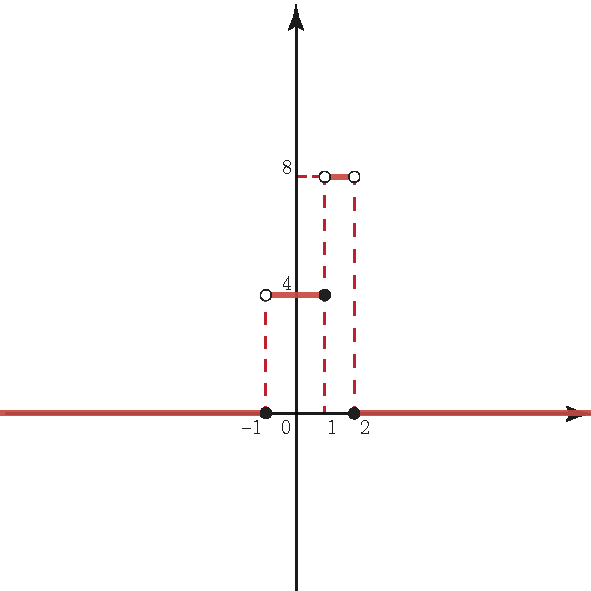
\includegraphics[trim=3cm 2cm 0cm 0cm, clip, scale=0.7]{images/graficosemplice.pdf}
		\end{minipage}\hspace{-7mm}
		\begin{minipage}{0.55\textwidth}
			Osserviamo che $s(x)=\left\{0,4,8\right\}$, dunque è semplice; le controimmagini dei valori $0$, $4$ e $8$ sono, rispettivamente:
			\begin{equation*}
				\begin{array}{l}
					A_1=s^{-1}\left(\left\{0\right\}\right)=\left(-\infty,-1\right]\cap\left[2,+\infty\right)\\
					A_2=s^{-1}\left(\left\{4\right\}\right)=\left(-1,1\right]\\
					A_3=s^{-1}\left(\left\{8\right\}\right)=\left(1,2\right)
				\end{array}
			\end{equation*}
		Pertanto la decomposizione standard di $s$ risulta
		\begin{align*}
			s&=0\chi_{\left(-\infty,-1\right]\cap\left[2,+\infty\right)}+4\chi_{\left(-1,1\right]}+8\chi_{\left(1,2\right)}=\\
			&=4\chi_{\left(-1,1\right]}+8\chi_{\left(1,2\right)}
		\end{align*}
		\end{minipage}\vspace{3mm}\\
	\item La funzione di Dirichlet
		\begin{equation*}
		s(x)=
		\begin{cases}
			\begin{array}{ll}
				1&\text{se }x\in\left[0,1\right]\cap\rationalset\\
				0&\text{se }x\in\left[0,1\right]\setminus\rationalset\\
			\end{array}
		\end{cases}
	\end{equation*}
	è semplice perché $s\left(\left[0,1\right]\right)=\left\{0,1\right\}$ e infatti $s=\chi_{\left[0,1\right]\cap\rationalset}$.
	\end{enumerate}
\end{examples}
\begin{minipage}{0.55\textwidth}
\subsection{Approssimazione di funzioni misurabili non negative con funzioni semplici}
Riprendendo l'idea di Lebesgue alla base del suo integrale, ci interessa studiare le funzioni passando attraverso la loro \textit{immagine}.\\
Si può ipotizzare di \textit{approssimare} tale funzione $f$ con una \textit{funzione semplice}: partizionando il codominio in opportuni intervalli individuati da quote fissate, se passiamo alle controimmagini possiamo sapere quali punti di $f$ sono contenuti nell'intervallo posto ad una certa quota e pertanto definire una funzione caratteristica che, come nelle \textit{carte topografiche a isoipse}, approssima la funzione $f$ per difetto.\\
Il prossimo teorema formalizza proprio questo ragionamento.
\end{minipage}\hspace{2mm}
\begin{minipage}{0.4\textwidth}
	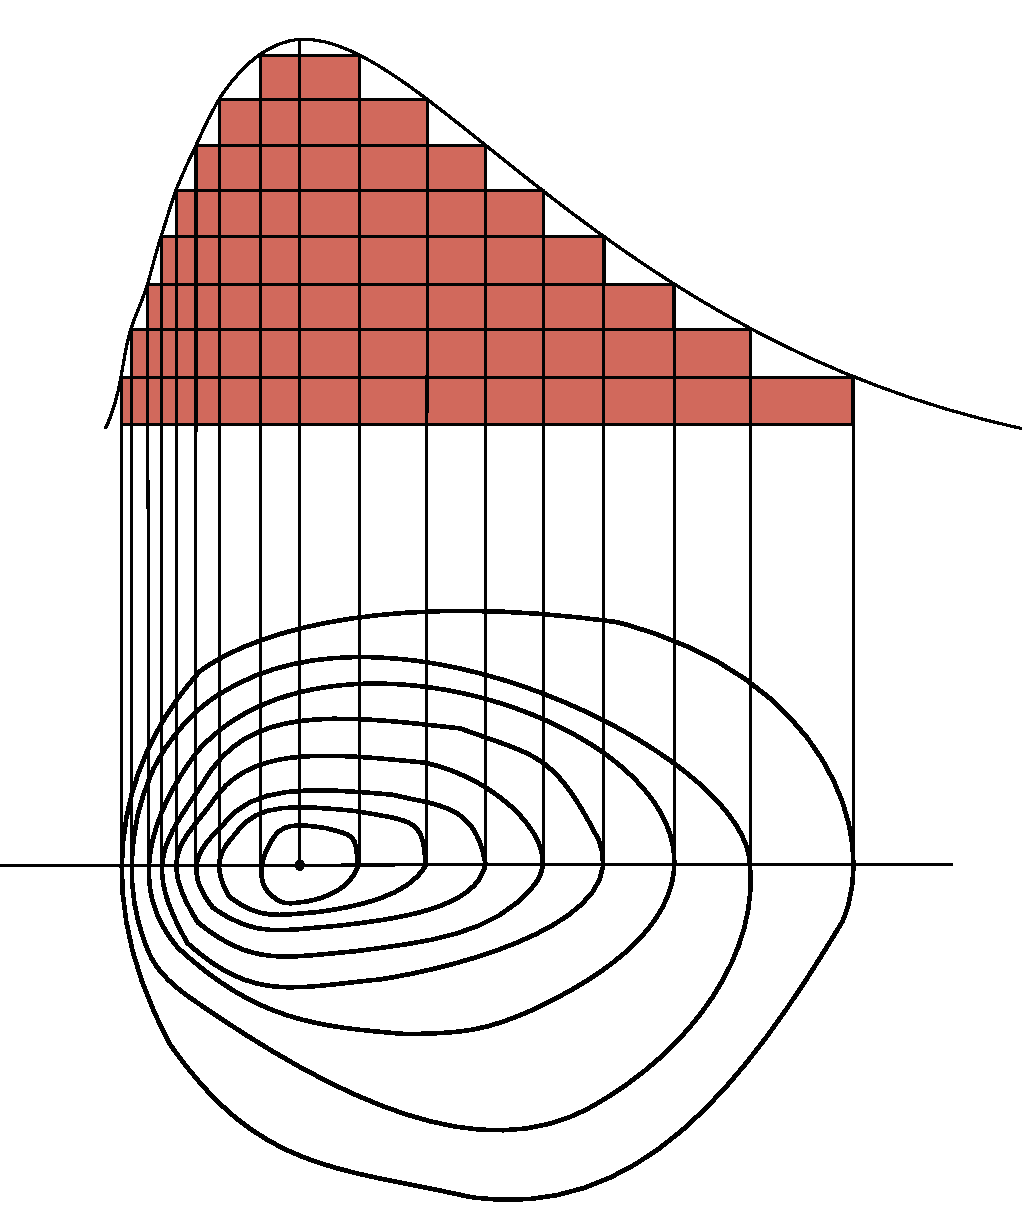
\includegraphics[trim=1cm 0cm 1.5cm 0cm, clip, scale=0.4]{images/isoipse}
\end{minipage}\vspace{3mm}\\
\begin{theorema}[Approssimazione di funzioni misurabili non negative con funzioni semplici]
	Sia $\left(X,\mathcal{M}\right)$ uno spazio misurabile e sia $\funz{f}{X}{\left[0,+\infty\right]}$ una funzione misurabile. Allora esiste una successione di funzioni semplici misurabili $\funz{s_n}{X}{\left[0,+\infty\right)}$ tale che
	\begin{itemize}
		\item $0\leq s_n(x)\leq s_{n+1}(x)\leq f(x),\ \forall x\in X,\ n\geq 1$.
		\item $\displaystyle\lim_{n\to+\infty}s_n(x)=f(x),\ \forall x\in X$.
	\end{itemize}
\end{theorema}
\begin{observe}
	La successione $s_n$ converge a $f$ puntualmente in modo \textit{monotono}.
\end{observe}
\begin{demonstration}~{}
	\begin{itemize}
		\item \textbf{\textsc{Passo 1}: costruzione della successione $s_n$ e verifica della monotonia.}\\
		Fissato $n\geq 1$, dividiamo $\left[0,+\infty\right)$ in $\left[0,n\right)$ e $\left[n,+\infty\right]$; dividiamo ulteriormente l'intervallo $\left[0,n\right)$ in $n2^n$ parti uguali
		\begin{equation*}
			\left[0,\frac{1}{2^n}\right)\quad\left[\frac{1}{2^n},\frac{2}{2^n}\right)\ldots\left[\frac{i-1}{2^n},\frac{i}{2^n}\right)\ldots\left[\frac{n2^n-1}{2^n},n\right),\ \forall i=1,\ \ldots,\ n2^n
		\end{equation*}
	Posto $E_{n,i}=f^{-1}\left(\left[\frac{i-1}{2^n},\frac{i}{2^n}\right)\right)$ e $F_n=f^{-1}\left(\left[n,+\infty\right]\right),\ \forall i=1,\ \ldots,\ n2^n$, si definisce
	\begin{equation}
		s_n=\sum_{i=1}^{n2^n}\frac{i-1}{2^n}\chi_{E_{n,i}}+n\chi_{F_n}
	\end{equation}
\begin{center}
	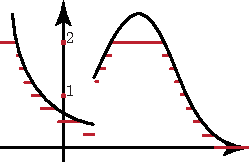
\includegraphics[trim=0cm 0cm 0cm 0cm, clip, scale=1.3]{images/approssimazione1}
\end{center}
Da questa costruzione segue che:
\begin{itemize}
	\item $s_n$ è semplice per $n$ fissato: è una combinazione lineare \textit{finita} di funzioni caratteristiche con pesi distinti.
	\item È monotona al crescere di $n$:\vspace{-3mm}
	\begin{equation*}
		0\leq s_n(x)\leq s_{n+1}(x)\leq f(x)\vspace{-3mm}
	\end{equation*}
	Intuitivamente, passando da $s_n$ a $s_{n+1}$:
	\begin{itemize}
		\item i nodi individuati in $s_n$ rimangono inalterati.
		\item vengono aggiunti dei nodi intermedi dimezzando ogni intervallino $\left[\frac{i-1}{2^n},\frac{i}{2^n}\right)$.
		\item vengono aggiunti dei nuovi nodi tra $n$ e $n+1$
	\end{itemize}
	Riducendo la dimensione di ciascun intervallino, l'approssimazione così definita risulta essere più raffinata del passo precedente; infatti, per ogni $x$ l'intervallo in cui sta ora $f(x)$ può avere lo stesso estremo inferiore che aveva con la partizione di $s_n$, oppure può avere un nuovo estremo inferiore dato da uno dei nodi introdotti con $s_{n+1}$.\\
\begin{minipage}{0.5\textwidth}
	\begin{center}
		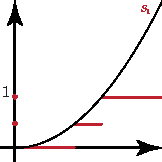
\includegraphics[trim=0cm 0cm 0cm 0cm, clip, scale=1.4]{images/approssimazione2}
	\end{center}
\end{minipage}
\begin{minipage}{0.5\textwidth}
	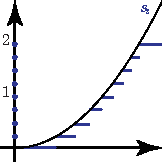
\includegraphics[trim=0cm 0cm 0cm 0cm, clip, scale=1.3]{images/approssimazione3}
\end{minipage}\vspace{4mm}
\end{itemize}
\item  \textbf{\textsc{Passo 2}: misurabilità di $s_n,\ \forall n\geq 1$.}\\
Ricordiamo che, dati $s_i\geq 0$ e $A_i\in\mathcal{M},\ i=1,\ \ldots,\ k$ si ha
\begin{equation*}
	s=\sum_{i=1}^{k}s_i\chi_{A_i}\text{ misurabile}\iff A_i\text{ misurabile},\ \forall i
\end{equation*}
Gli intervalli di $\left[\frac{i-1}{2^n},\frac{i}{2^n}\right),\ \forall i=1,\ \ldots,\ n2^n$ e $\left[n,+\infty\right)$ sono Boreliani in $\left[0,+\infty\right]$; pertanto, le controimmagini $E_{n,i}$ e $F_n$ tramite $f$ funzione misurabile sono anch'esse misurabili in $X$.
\item  \textbf{\textsc{Passo 3}: approssimazione nel senso della convergenza puntuale.}\\
	Proviamo che vale la relazione
	\begin{equation*}
		\lim_{n\to+\infty}s_n(x)=f(x),\ \forall x\in\ X
	\end{equation*}
Fissiamo $x\in X$ e distinguiamo i casi.
\begin{itemize}
	\item \textbf{\textsc{Caso 1:}} $f(x)\in\left[0,+\infty\right)$.\\
	Poiché $\floor{f(x)}\leq f(x)<\floor{f(x)}+1$, posto $N_x\coloneqq \floor{f(x)}+1$ si ha che
	\begin{equation*}
		f(x)< N_x\leq n,\ \forall n\geq N_x
	\end{equation*}
Pertanto, esiste $N_x\geq 1$ tale per cui $f(x)<n,\ \forall n\geq N_X$.\\
Sulla base di ciò si ha che $f(x)\in\left[0,n\right),\ \forall n\geq N_x$ e dunque esiste $i\in\left\{0,\ldots,n2^n\right\}$ tale per cui
\begin{equation*}
	f(x)\in\left[\frac{i-1}{2^n},\frac{i}{2^n}\right)\implies x\in f^{-1}\left(\left[\frac{i-1}{2^n},\frac{i}{2^n}\right]\right)=E_{n,i}
\end{equation*}
Allora $s_n(x)=\frac{i-1}{2^n}$ perché
\begin{gather*}
	\chi_{E_{n,j}}(x)=\delta_{i,j}\\
	\chi_{F_n}(x)\equiv 0
\end{gather*}
dove $\delta_{i,j}$ è il delta di Kronecker; segue che
\begin{equation*}
	0\leq s_n(x)=\frac{i-1}{2^n}\leq f(x)< \frac{i}{2^n}\implies 0\leq f(x)-s_n(x)<\frac{i}{2^n}
\end{equation*}
Passando al limite
\begin{equation*}
	0\leq \lim_{n\to+\infty}f(x)-s_n(x)\leq \lim_{n\to+\infty}\frac{i}{2^n}=0
\end{equation*}
Pertanto, per il \textit{teorema del confronto}
\begin{equation*}
	\lim_{n\to+\infty}f(x)-s_n(x)=0\implies \lim_{n\to+\infty}s_n(x)=f(x).
\end{equation*}
\item \textbf{\textsc{Caso 2:}} $f(x)=+\infty$.\\
Chiaramente
\begin{equation*}
	f(x)\in\left[n,+\infty\right],\ \forall n\geq 1\implies x\in f^{-1}\left(\left[n,+\infty\right]\right)=F_n
\end{equation*}
Allora $s_n(x)=n$ perché
\begin{gather*}
	\chi_{E_{n,j}}(x)\equiv 0\\
	\chi_{F_n}(x)\equiv 1
\end{gather*}
Segue che
\begin{equation*}
	\lim_{n\to+\infty}s_n(x)=\lim_{n\to+\infty}n=+\infty=f(x)\implies \lim_{n\to+\infty}s_n(x)=f(x)\qedhere
\end{equation*}
\end{itemize}
\end{itemize}
\end{demonstration}

\section{Passo 1: funzioni semplici, misurabili, non negative}
\begin{define}[Integrale di Lebesgue per funzioni semplici, misurabili, non negative]
	Sia $\funz{s}{\left(X,\mathcal{M},\mu\right)}{\left[0,+\infty\right)}$ funzione semplice, misurabile e non negativa che si decompone, dato $s(x)=\left\{\alpha_1,\ldots, \alpha_n\right\}$, nella forma standard
	\begin{equation*}
		s=\sum_{i=1}^{n}\alpha_i\chi_{A_i}\quad A_i=s^{-1}\left(\left\{A_i\right\}\right)
	\end{equation*}
	Dato $E\in\mathcal{M}$, si definisce \textit{integrale esteso a $A$ di $s$ rispetto alla misura $\mu$} il valore
	\begin{equation}
		\int_{E}sd\mu\coloneqq\sum_{i=1}^{n}\alpha_i\mu\left(A_i\cap E\right)
	\end{equation}
	con la convenzione che se un termine di tale sommatoria è $0\cdot \infty$ allora tale termine sia uguale a $0$.
\end{define}
\begin{observe}
	$\mu\left(A_i\cap E\right)$ è ben definito in quanto $A_i\cap E$ è misurabile:
	\begin{itemize}
		\item $A_i$ sono misurabili $\forall i$ perché $s$ è misurabile per ipotesi.
		\item $E$ è misurabile per ipotesi.
		\item L'\textit{intersezione} è un'operazione chiusa nella $\sigma$-algebra $\mathcal{M}$
	\end{itemize}
\end{observe}
\begin{observe}
	Come mai poniamo convenzionalmente $0\cdot \infty=0$? L'integrale generalizza e astrae il calcolo dell'area sottesa ad una curva; se ho un intervallo di lunghezza infinita ma a quota zero, chiaramente l'area sottesa è uguale a zero.
\end{observe}
\begin{examples} Per il primo e secondo esempio riprendiamo le funzioni viste a pag. \pageref{funzionesemplice}.
	\begin{enumerate}
		\item Consideriamo la funzione del primo esempio, che ha dominio in $\left(\realset^n,\mathcal{L}(\realset),m_1\right)$ e calcoliamo l'integrale su $E=\realset$:
		\begin{equation*}
			\begin{array}{ll}
				\displaystyle	\int_{\realset}sdm_1&=0m_1\left(\left(-\infty,-1\right]\cup\left[2,+\infty\right)\right)+4m_1\left(\left[-1,1\right]\right)+8m_2\left(\left(1,2\right)\right)=\\
				&=0\cdot\left(+\infty\right)+4\cdot 2+8\cdot 1=16
			\end{array}
		\end{equation*}
		\item \label{funzionedirichletintegrale}Consideriamo la funzione di Dirichlet su $\left[0,1\right]$, che ha dominio in $\left(\realset,\mathcal{L}(\realset),m_1\right)$  l'integrale su $E=\left[0,1\right]$:
		\begin{equation*}
			\int_{\left[0,1\right]}sdm_1=1\cdot m_1\left(\left[0,1\right]\cap\rationalset\right)+0\cdot m_1\left(\left[0,1\right]\setminus\rationalset\right)
		\end{equation*}
	Poiché
	\begin{itemize}
		\item $\left[0,1\right]\cap \rationalset$ è misurabile e si ha $m_1\left(\left[0,1\right]\cap \rationalset\right)=0$.
		\item $m_1\left(\left[0,1\right]\setminus\rationalset\right)=m1\left(\left[0,1\right]\right)-m1\left(\left[0,1\right]\cap\rationalset\right)=1-0=1$
	\end{itemize}
	allora
	\begin{equation*}
		\int_{\left[0,1\right]}sdm_1=1\cdot 0+0\cdot 1=0
	\end{equation*}
\item Consideriamo $\left(X,\mathcal{M},\mu\right)=\left(\naturalset,\setpart{\naturalset},\mu_p\right)$ con $\mu_p$ la misura di conteggio di \textbf{Poisson} di parametro $\lambda>0$:\index{misura!di conteggio!di Poisson}.
\begin{gather}
	\mu_p\left(\left\{n\right\}\right)=e^{-\lambda}\frac{\lambda^n}{n!}, \forall n\geq 0\\
	\mu_p\left(E\right)=\sum-{n\colon n\in E}e^{-\lambda}\frac{\lambda^n}{n!}, \forall E\subseteq \naturalset
\end{gather}
Definiamo $\funz{s}{\naturalset}{\left[0,+\infty\right)}$ come
\begin{equation*}
	s\left(n\right)=\begin{cases}
		\begin{array}{ll}
			1&\text{se }n=0,1\\
			2&\text{se }n\geq 2
		\end{array}
	\end{cases}
\end{equation*}
La funzione $s$ è semplice, dato che $s\left(\naturalset\right)=\left\{1,2\right\}$, e
\begin{equation*}
	s=\chi_{\left\{0,1\right\}}+2\chi_{\left\{n\in\naturalset\mid n\geq 2\right\}}
\end{equation*}
Allora, posto $E=\naturalset$, l'integrale sul dominio è
\begin{equation*}
\begin{array}{ll}
	\displaystyle\int_{\naturalset}sd\mu_P&=1\cdot \mu_P\left(\left\{0,1\right\}\right)+2\mu_P\left(\left\{n\in\naturalset\mid n\geq 2\right\}\right)=\\
	&\displaystyle=e^{-\lambda}\cdot 1+e^{-\lambda}\frac{\lambda}{1}+2\sum_{n\geq 2}e^{-\lambda}\frac{\lambda^n}{n!}=\\
	&\displaystyle=e^{-\lambda}+\lambda e^{-\lambda}+2\sum_{n\geq 2}e^{-\lambda}\frac{\lambda^n}{n!}
\end{array}
\end{equation*}
	\end{enumerate}
\end{examples}
\begin{observe}
	La funzione di Dirichlet è una funzione \textit{non} integrabile secondo \textit{Riemann}, ma è integrabile secondo Lebesgue.
\end{observe}
\subsection{{$\sigma$}-additività dell'integrale di funzioni semplici, misurabili, non negative rispetto al dominio}
\begin{proposition}[{$\sigma$}-additività dell'integrale di funzioni semplici, misurabili, non negative rispetto al dominio]
	Sia $\left(X,\mathcal{M},\mu\right)$ uno spazio di misura e sia $\funz{s}{X}{\left[0,+\infty\right)}$ semplice misurabile \textit{non} negativa. Allora vale
	\begin{equation}
		\int_{\union_{n\geq 1}E_n}sd\mu=\sum_{n\geq 1}\int_{E_n}sd\mu,\ \forall E_n\in\mathcal{M}\colon E_i\cap E_j=\emptyset,\ \forall i\neq j
	\end{equation}
\end{proposition}
Per dimostrare tale proprietà ci servirà un risultato sulle serie con \textit{doppi indici}.
\begin{propositionsqed}[Commutatività degli indici nelle serie doppie]~\label{commutativitàindici}
	\begin{itemize}
		\item Se $a_{ij}\geq0\ \forall i,j$, allora
		\begin{equation*}
			\sum_{i=1}^{+\infty}\sum_{j=1}^{+\infty}a_{ij}=\sum_{j=1}^{+\infty}\sum_{i=1}^{+\infty}a_{ij}
		\end{equation*}
		\item Più in generale, se $\displaystyle\sum_{i=1}^{+\infty}\sum_{j=1}^{+\infty}\abs{a_{ij}}<+\infty$, allora vale la relazione precedente.\qedhere
	\end{itemize}
\end{propositionsqed}
\begin{demonstrationwt}[della {$\sigma$}-additività dell'integrale rispetto al dominio]
	Siano $E_n\in\mathcal{M},\ E_i\cap E_j= \emptyset$ e sia $\displaystyle E=\cup_{n\geq 1} E_n$. Sia $\displaystyle s=\sum_{i=1}^{k}\alpha_i\chi_{A_i}$ la decomposizione standard di $s$ funzione semplice, dove $s(x)=\left\{\alpha_1,\ldots,\alpha_k\right\}$ e $A_i=s^{-1}\left(\left\{\alpha_i\right\}\right),\ \forall i=1,\ \ldots,\ k$. Si ha
	\begin{equation*}
		\int_Esd\mu=\sum_{i=1}^{k}\alpha_i\mu\left(A_i\cap E\right)\squarequal
	\end{equation*}
	Per $\sigma$-additività della misura $\mu$ vale
	\begin{equation*}
		\mu\left(A_i\cap E\right)=\sum_{j=1}^{+\infty}\mu\left(A\cap E_j\right)
	\end{equation*}
quindi
\begin{equation*}
	\squarequal \sum_{i=1}^{k}\alpha_i\sum_{j=1}^{+\infty}\mu\left(A_i\cap E_j\right)=\sum_{i=1}^{k}\sum_{j=1}^{+\infty}\underbrace{\alpha_i\mu\left(A_i\cap E_j\right)}_{\geq 0}=\sum_{j=1}^{+\infty}\sum_{i=1}^{k}\alpha_i\mu\left(A_i\cap E_j\right)=\sum_{j=1}^{+\infty}\int_{E_j}sd\mu
\end{equation*}
\end{demonstrationwt}
Vediamo il risultato appena dimostrato da un punto di vista differente. Possiamo considerare l'integrale di Lebesgue non solo come un \textit{funzionale} che, fissato un insieme misurabile $E\in\left(X,\mathcal{M},\mu\right)$, agisce sulla funzione $s$, bensì come una \textit{funzione d'insieme} in cui $s$ è fissata, mentre la variabile è l'insieme misurabile $E$:
\begin{equation}
	\funztot{\mu_s}{\mathcal{M}}{\left[0,+\infty\right]}{E}{\int_Esd\mu}
\end{equation}
L'uguaglianza ricavata dalla proposizione precedente 
\begin{equation*}
	\int_{\cup_{n\geq 1}E_n}sd\mu=\sum_{n\geq 1}\int_{E}sd\mu,\ \forall E_n\in\mathcal{M}\colon E_i\cap E_j=\emptyset,\ \forall i\neq j
\end{equation*}
si riscrive pertanto come
\begin{equation*}
	\mu_s\left(\bigcup_{n\geq 1}E_n\right)=\sum_{n\geq 1}\mu_s\left(E_n\right)
\end{equation*}
Pertanto, $\mu_s$ è una misura su $\mathcal{M}$.
\section{Passo 2: funzioni a valori reali misurabili, non negative}
Sia $\funz{f}{\left(X,\mathcal{M},\mu\right)}{\left[0,+\infty\right]}$ funzione misurabile e non negativa. Dato $E\in\mathcal{M}$, vogliamo definire l'\textit{integrale esteso ad E di $f$ rispetto alla misura $\mu$} utilizzando l'integrale delle funzioni semplici definito al passo 1. 
\begin{define}[Integrale di Lebesgue per funzioni a valori reali, misurabili, non negative]
	Sia $\funz{f}{\left(X,\mathcal{M},\mu\right)}{\left[0,+\infty\right]}$ funzione misurabile e non negativa. Si definisce l'\textit{integrale esteso ad E di $f$ rispetto alla misura $\mu$} come
	\begin{equation}
		\int_Efd\mu\coloneqq\sup\left\{\int_Esd\mu\ \middle| \funz{s}{X}{\left[0,+\infty\right)}\text{ semplice, misurabile}\colon0\leq s\leq f\right\}
	\end{equation}
\end{define}
\begin{observe}~{}
	\begin{itemize}
		\item L'insieme
		\begin{equation*}
			\left\{\int_Esd\mu\ \middle|\funz{s}{X}{\left[0,+\infty\right)}\text{ semplice, misurabile}\colon0\leq s\leq f\right\}\subseteq \left[0,+\infty\right]
		\end{equation*} non è vuoto, in quanto contiene sempre $0=\int_E 0d\mu$.
		\item $\int_Efd\mu\in\left[0,+\infty\right]$
		\item Se $f$ è semplice allora si ritrova l'integrale definito al \textit{passo 1}.
	\end{itemize}
\end{observe}
\begin{attention}~{}\\
	\textbf{Ogni funzione misurabile \textit{non negativa} ammette integrale secondo Lebesgue.}\\
	Questa notevole differenza rispetto all'integrale di Riemann è situa nella definizione. Se l'integrale di Riemann richiede che la somma inferiore e la somma superiore coincidono, quello di Lebesgue richiede solo l'esistenza del $\sup$: la prima condizione non si verifica sempre, mentre la seconda è sempre verificata in $\realset^{\ast}$.
\end{attention}
\begin{property}[Proprietà dell'integrale di Lebesgue per funzioni misurabili non negative]
	Sia $\left(X,\mathcal{M},\mu\right)$ uno spazio di misura.
	\begin{enumerate}
		\item \textbf{Monotonia rispetto alla funzione integranda:}\\
		date $\funz{f,g}{X}{\left[0,+\infty\right]}$ misurabili, non negative tali per cui $f\leq g$, allora
		\begin{equation}
			\int_E fd\mu\leq \int_E gd\mu,\ \forall E\in\mathcal{M}
		\end{equation}
		\item \textbf{Monotonia rispetto al dominio della funzione integranda:}\\
		dati $\funz{f}{X}{\left[0,+\infty\right]}$ misurabile, non negativa e $E,\ F\in\mathcal{M}$ tali per cui $E\subseteq F$, allora
		\begin{equation}
			\int_Efd\mu\leq \int_Fgd\mu
		\end{equation}
		\item \textbf{Linearità dell'integrale (prodotto per uno scalare):}\\
		dati $\funz{f}{X}{\left[0,+\infty\right]}$ misurabile, non negativa e $c\geq 0$
		\begin{equation}
			\int_E cfd\mu=c\int_Efd\mu,\ \forall E\in\mathcal{M}
		\end{equation}
		\item \textbf{Ininfluenza degli insiemi di misura nulla sull'integrale:}\\
		sia $\funz{f}{X}{\left[0,+\infty\right]}$ misurabile, non negativa; se $E\in\mathcal{M}$ con $\mu\left(E\right)=0$, allora
		\begin{equation}
			\int_Efd\mu=0
		\end{equation}
		\item \textbf{Integrazione sullo spazio intero:}\\
		sia $\funz{f}{X}{\left[0,+\infty\right]}$ misurabile, non negativa; allora
		\begin{equation}
			\int_E fd\mu=c\int_Xf\chi_Ed\mu,\ \forall E\in\mathcal{M}
		\end{equation}
	\end{enumerate}
\end{property}
\subsection{Teorema della convergenza monotona}
Il \textbf{teorema della convergenza monotona}\index{teorema!della convergenza monotona}, altresì noto come \textbf{Teorema di Beppo Levi}\seeonlyindex{teorema!di Beppo Levi}{teorema!della convergenza monotona} (principalmente in Italia) o di \textbf{Lebesgue}\seeonlyindex{teorema!di Lebesgue}{teorema!della convergenza monotona}, si inserisce nel filone dei risultati sul problema del \textit{passaggio al limite sotto segno di integrale} di cui abbiamo parlato per la prima volta nel \refChapterOnly{ellipseintroduction}.\\
Abbiamo già visto\footnote{Si veda \refChapterOnly{seriefunzioni}, teorema \ref{passaggioallimitecontinuitàuniforme}, pag. \pageref{passaggioallimitecontinuitàuniforme}.} che se una successione di funzioni $f_n$ Riemann-integrabili su un compatto converge uniformemente a $f$, allora $f$ è Riemann-integrabile e vale il passaggio al limite dell'integrale. Il teorema che dimostreremo, pur essendo applicabile solo a funzioni misurabili e monotone \textit{crescenti}, risulta avere diversi notevoli vantaggi rispetto al risultato basato sulla convergenza uniforme.
\begin{theorema}[Teorema della convergenza monotona]\label{thmconvergenzamonotona}
	Siano $\left(X,\mathcal{M},\mu\right)$ uno spazio di misura e $\funz{f_n,f}{X}{\left[0,+\infty\right]}$ con $n\geq 1$ tali che
	\begin{enumerate}
		\item $f_n$ sono misurabili.
		\item $\displaystyle\lim_{n\to+\infty}f_n(x)=f(x),\ \forall x\in X$.
		\item $0\leq f_n(x)\leq f_{n+1}(x),\ \forall n\geq 1,\ \forall x\in X$.
	\end{enumerate}
allora
\begin{enumerate}
	\item $f$ è misurabile.
	\item Vale il \textbf{passaggio al limite sotto segno di integrale}\index{passaggio al limite sotto segno di integrale}:
	\begin{equation}
		\lim_{n\to+\infty}\int_Xf_nd\mu=\int_Xfd\mu\in\left[0,+\infty\right]
	\end{equation}
\end{enumerate}
\end{theorema}
\begin{observes}~{}
	\begin{itemize}
		\item L'uguaglianza della tesi è valida per ogni misura di $X$, anche infinita.
		\item Il risultato è in generale \textit{falso} se $f_n(x)$ decresce rispetto ad $n,\ \forall x\in X$.
	\end{itemize}
\end{observes}
\begin{examplewt}[Controesempio con una successione di funzioni decrescenti]
	Sia $\left(X,\mathcal{M},\mu\right)=\left(\realset,\mathcal{L}(\realset),m_1\right)$ e $f_n(x)=\frac{1}{n},\ \forall x\in\realset$. Per ogni $x$ vale
	\begin{itemize}
		\item $f_n(x)$ decrescente rispetto ad $n$.
		\item $\displaystyle\lim_{n\to+\infty}f_n(x)=0$
	\end{itemize}
Pertanto:
\begin{align*}
	\lim_{n\to+\infty}\int_{\realset}f_ndm_1=\lim_{n\to+\infty}\left(+\infty\right)&=+\infty\\
	\int_{\realset}\left(\lim_{n\to+\infty}f_n\right)dm_1=\int_{\realset}0dm_1&=0
\end{align*}
\end{examplewt}
\begin{demonstrationcaputwt}[del teorema della convergenza monotona]~
	\begin{enumerate}[label=\Roman*]
		\item $f$ è misurabile perché è limite puntuale di funzioni misurabili.
		\item Osserviamo che $f$ misurabile e non negativa implica che
		\begin{equation*}
			\exists\int_Xfd\mu\in\left[0,+\infty\right]
		\end{equation*}
		Dalla monotonia data per ipotesi 3) segue, per monotonia dell'integrale rispetto alla funzione integranda, che
	\begin{equation*}
		0\leq\lefteqn{\underbrace{\phantom{\int_Xf_nd\mu\leq\int_Xf_{n+1}d\mu}}_{\circled[red]{\vardiamond}}}\int_Xf_nd\mu\leq
		\overbrace{\int_Xf_{n+1}d\mu\leq \int_Xfd\mu}^{\circled[blue]{\spadesuit}}
	\end{equation*}
		Da \circled[red]{\vardiamond} si nota come la successione
	\begin{equation*}
		\int_Xf_nd\mu\in\left[0,+\infty\right]
	\end{equation*}
		è crescente e quindi per il \textit{teorema sui limiti di successioni monotone} esiste il suo limite
\begin{equation*}
	\lim_{n\to+\infty}\int_Xf_nd\mu\in\left[0,+\infty\right]
\end{equation*}
Considerando \circled[blue]{\spadesuit}, per il \textit{teorema della permanenza del segno} si ottiene
\begin{equation*}
	\lim_{n\to+\infty}\int_Xf_nd\mu\leq \int_Xfd\mu
\end{equation*}
È sufficiente dimostrare che vale la disuguaglianza di verso opposto:
\begin{equation*}
	\lim_{n\to+\infty}\int_Xf_nd\mu\geq \int_Xfd\mu
\end{equation*}
Ricordiamo che per definizione
\begin{equation*}
	\int_Xfd\mu=\sup\left\{\int_Xsd\mu\middle| \funz{s}{X}{\left[0,+\infty\right)}\text{ semplice, misurabile}\colon0\leq s\leq f\right\}
\end{equation*}
Pertanto ci sarà sufficiente provare che
\begin{equation*}
	\lim_{n\to+\infty}\int_Xf_nd\mu\geq \int_Xsd\mu,\ \forall s\text{ funzione definita come sopra.}
\end{equation*}
Osserviamo che questa è vera se mostriamo che
\begin{equation*}
	\lim_{n\to+\infty}\int_Xf_nd\mu\geq c\int_Xsd\mu,\ \forall s\text{ funzione definita come sopra},\ \forall c\in\left(0,1\right)
\end{equation*}
Basterà infatti passare poi al limite per $c\to 1^{-}$ per ottenere la condizione cercata.\\
Siano quindi $c\in\left(0,1\right)$ e $\funz{s}{X}{\left[0,+\infty\right]}$ semplice, misurabile e tale che $0\leq s\leq f$ su $X$. Per ogni $n\geq 1$ definiamo
\begin{equation*}
	E_n=\left\{x\in X\mid f_n(x)\geq cs(x)\right\}
\end{equation*}
Osserviamo che se $x\in\ E_n$, allora
\begin{equation*}
	f_n(x)\geq cs(x)\implies f_{n+1}(x)\geq f_n(x)\geq cs(x)\implies x\in E_{n+1},\ \forall n\geq 1,
\end{equation*}
cioè $E_n\subseteq E_{n+1},\ \forall n\geq 1$.
Ora abbiamo
\begin{equation*}
	\int_Xf_nd\mu\geq \int_{E_n}f_nd\mu\geq \int_{E_n}csd\mu=c\int_Esd\mu=c\mu_s\left(E_n\right)
\end{equation*}
dove $\mu_s$ è la misura definita come 
\begin{equation*}
	\mu_s\left(E\right)=\int_Esd\mu
\end{equation*}
Abbiamo quindi ricavato che
\begin{equation*}
	\circled[green]{\clubsuit}\int_Xf_nd\mu\geq c\mu_s\left(E_n\right),\ \forall n\geq 1
\end{equation*}
Se $n\to+\infty$, essendo $\mu_S$ una misura $E_n$ una successione insiemistica crescente, per continuità della misura
\begin{equation*}
	\lim_{n\to+\infty}\mu_s\left(E_n\right)=\mu_s\left(\bigcup_{n\geq 1}E_n\right)
\end{equation*}
Passando al limite nella disequazione \circled[green]{\clubsuit} otteniamo
\begin{equation*}
	\lim_{n\to+\infty}\int_Xf_nd\mu\geq c\mu_s\left(\bigcup_{n\geq 1}E_n\right)=c\int_{\bigcup_{n\geq 1}E_n}d\mu_s
\end{equation*}
Per concludere, proviamo che
\begin{equation*}
	\bigcup_{n\geq 1}E_n=X
\end{equation*}
Banalmente l'inclusione $\subseteq$ è verificata; per trovare l'altra si usa la convergenza puntuale di $f_n(x)$ e $f(x),\ \forall x\in X$. Poiché $f_n$ è una successione di funzioni crescenti e con limite puntuale a $f$ su $X$, sappiamo che $f_n\leq f$ e quindi
\begin{equation*}
	f(x)\geq f_n(x)\geq cs(x)
\end{equation*}
Prendiamo ora $x\in X$: se $f(x)=0$, allora $x\in E_1$ in quanto segue che $s(x)=0$; se $f(x)>0$, allora $x\in E_n$ per qualche $n$.
\qedhere
\end{enumerate}
\end{demonstrationcaputwt}
\subsection{Additività dell'intergrale, scambio di integrale e serie}
\begin{proposition}[Additività dell'integrale]
	Sia $\left(X,\mathcal{M},\mu\right)$ uno spazio di misura e siano $\funz{f_1,\ \ldots,\ f_N}{X}{\left[0,+\infty\right]}$ funzioni misurabili. Allora
	\begin{equation}
		\int_X \left(\sum_{i=1}^{N}f_i\right)d\mu=\sum_{i=1}^{N}\int_Xf_id\mu
	\end{equation}
\end{proposition}
\begin{observe}
	\textit{Tutti} gli integrali nell'enunciato esistono (eventualmente infiniti) in quanto le $f_i$ sono funzioni misurabili non negative.
\end{observe}
\begin{demonstration}
	Si prova per induzione su $N$. Il passo induttivo è immediato, pertanto proviamo la base dell'induzione ($N=2$): dimostriamo dunque che
	\begin{equation*}
		\int_X\left(f_1+f_2\right)d\mu=\int_Xf_1d\mu+\int_Xf_2d\mu
	\end{equation*}
		\begin{itemize}
		\item \textbf{\textsc{Passo 1}:} proviamo il risultato nel caso di funzioni semplici $\funz{s,t}{X}{\left[0,+\infty\right)}$ misurabili. Esse si possono scrivere come
		\begin{equation*}
			\begin{array}{lll}
				& \displaystyle s=\sum_{i=1}^{k}s_i\chi_{A_i} & \displaystyle t=\sum_{i=1}^n{k}t_j\chi_{B_j}\\
				\text{dove}& \displaystyle s(x)=\left\{s_1,\ldots,s_k\right\}&\displaystyle t(x)=\left\{t_1,\ldots,t_n\right\}\\
				&\displaystyle A_i=s^{-1}\left(\left\{s_i\right\}\right),\ i=1,\ldots,\ k&\displaystyle B_j=t^{-1}\left(\left\{t_j\right\}\right),\ j=1,\ldots,\ n\\
			\end{array}
		\end{equation*}
	Consideriamo $E_{i,j}=A_i\cap B_j,\ \forall i,\ \ldots,\ k$ e $j=1,\ \ldots,\ n$: essi formano una nuova partizione di $X$ e, preso $x\in E_{ij}$, si ha
	\begin{equation*}
		\begin{cases}
			s(x)=s_i\\
			t(x)=t_j
		\end{cases}
	\end{equation*}
\begin{center}
	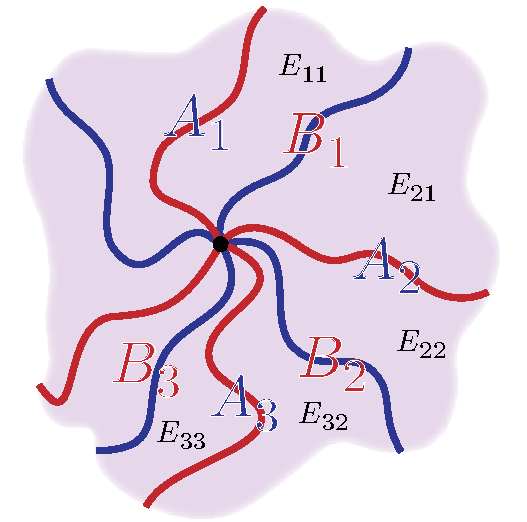
\includegraphics[trim=0cm 0cm 0cm 0cm, clip, scale=0.75]{images/additivita}
\end{center}
	Questo significa che $s(x)+t(x)=s_i+t_j,\ \forall x\in E_{ij}$, ossia
	\begin{equation*}
		s+t=\sum_{i,j}\left(s_i+t_j\right)\chi_{E_{ij}}
	\end{equation*}
	Integriamo secondo Lebesgue:
	\begin{equation*}
		\int_X\left(s+t\right)d\mu=\sum_{i,j}\left(s_i+t_j\right)\mu\left(E_{ij}\right)=\sum_{i,j}s_i\mu\left(E_{ij}\right)+\sum_{i,j}t_j\mu\left(E_{ij}\right)=\int_Xsd\mu+\int_Xtd\mu
	\end{equation*}
	\item \textbf{\textsc{Passo 2}:} proviamo il risultato nel caso di funzioni $\funz{f_1,f_2}{X}{\left[0,+\infty\right)}$ misurabili.\\
	È noto che:
	\begin{itemize}
		\item Esiste una successione di funzioni semplici misurabili $\funz{s_n}{X}{\left[0,+\infty\right]}$ tali che
		\begin{itemize}
			\item $0\leq s_n(x)\leq s_{n+1}(x)\leq f_1(x),\ \forall x\in X$.
			\item $\displaystyle \lim_{n\to+\infty}s_n(x)=f_1(x),\ \forall x\in\ X$
		\end{itemize}
		\item Esiste una successione di funzioni semplici misurabili $\funz{t_n}{X}{\left[0,+\infty\right]}$ tali che
		\begin{itemize}
			\item $0\leq t_n(x)\leq t_{n+1}(x)\leq f_2(x),\ \forall x\in X$.
			\item $\displaystyle \lim_{n\to+\infty}t_n(x)=f_2(x),\ \forall x\in\ X$
		\end{itemize}
	\end{itemize}
	Di conseguenza si ha
	\begin{align*}
		0\leq \left(s_n+t_n\right)(x)\leq \left(s_{n+1}+t_{n+1}\right)(x)\leq\left(f_1+f_2\right)(x),\ \forall x\in\ X\\
		\lim_{n\to+\infty}\left(s_n+t_n\right)(x)=\left(f_1+f_2\right)(x),\ \forall x\in\ X
	\end{align*}
	Integriamo secondo Lebesgue:
	\begin{align*}
		\int_X \left(f_1+f_2\right)d\mu&=\lim_{n\to+\infty}\int_X\left(s_n+t_n\right)d\mu&\text{(thm. conv. monotona)}\\
		&=\lim_{n\to+\infty}\left(\int_Xs_nd\mu+\int_Xt_nd\mu\right)&\text{(passo 1)}\\
		&=\lim_{n\to+\infty}\int_Xs_nd\mu+\lim_{n\to+\infty}\int_Xt_nd\mu&\\
		&=\int_Xf_1d\mu+\int_Xf_2d\mu&\text{(thm. conv. monotona)\qedhere}
	\end{align*}
	\end{itemize}
\end{demonstration}
Una conseguenza immediata di questa proprietà è che per le successioni di funzioni misurabili non negative vale lo \textit{scambio tra integrale e serie}.
\begin{corollary}[Scambio tra integrale e serie per funzioni misurabili e non negative]
Sia $\left(X,\mathcal{M},\mu\right)$ uno spazio di misura siano $\funz{f_n}{X}{\left[0,+\infty\right]},\ n\geq 1$ funzioni misurabili. Allora vale lo scambio tra integrale e serie:\index{scambio tra integrale e serie}
	\begin{equation}
		\int_X\left(\sum_{n=1}^{+\infty}f_n\right)d\mu=\sum_{n=1}^{+\infty}\int_Xf_nd\mu
	\end{equation}
\end{corollary}
\begin{demonstration}
	Consideriamo la successione delle ridotte
	\begin{equation*}
		g_k(x)=\sum_{n=1}^{k}f_n(x),\ \forall x\in X.
	\end{equation*}
	Ricordiamo che $g_k(x)$ è una successione crescente su $k$ per ogni $x\in X$, in quando $f_n(x)\geq 0$; poiché valgono le ipotesi del \textit{teorema della convergenza monotona} sulla successione $g_k$, possiamo applicarlo.\\
	Prima di farlo, osserviamo che per additività dell'integrale vale
	\begin{equation*}
		\int_X \sum_{n=1}^{k}f_n=\sum_{n=1}^{k}\int_X f_n
	\end{equation*}
	Noto ciò, dimostriamo facilmente il risultato desiderato: 
	\begin{align*}
		&\int \left(\lim_{k\to+\infty}g_k\right)d\mu=\lim_{k\to+\infty}\int_X g_kd\mu\\
		&\implies \int \left(\lim_{k\to+\infty}\sum_{n=1}^{k}f_n\right)d\mu=\lim_{k\to+\infty}\int_X \sum_{n=1}^{k}f_nd\mu=\lim_{k\to+\infty}\sum_{n=1}^{k}\int_X f_n\\
		&\implies \int_X\left(\sum_{n=1}^{+\infty}f_n\right)d\mu=\sum_{n=1}^{+\infty}\int_Xf_nd\mu\qedhere
	\end{align*}
\end{demonstration}
\subsection{Integrazione rispetto alla misura conteggio pesata}
\begin{theorema}[Integrazione rispetto alla misura conteggio pesata]\label{integrazionemisuraconteggiopesata}
	Sia $\left(\naturalset,\setpart{\naturalset},\mu_p\right)$ spazio di misura dove $\mu_p$ è la \textit{misura conteggio pesata} definita da
	\begin{align*}
		\mu_p\left(\left\{n\right\}\right)=p_n,\ \forall n\geq 1\text{ con }p_n\geq 0\\
		\mu_p\left(E\right)=\sum_{n\geq E}\mu_p\left(\left\{n\right\}\right),\ \forall E\subseteq \naturalset
	\end{align*}
Sia $\funz{f}{\naturalset}{\left[0,+\infty\right]}$. Allora si ha
\begin{equation*}
	\int_{\naturalset}fd\mu_p=\sum_{n\geq 1}f_np_n
\end{equation*}
In particolare, se $p_n=1,\ \forall n\geq 1$, si ha, indicata con $\mu^{\ast}$ la misura conteggio corrispondente,
\begin{equation*}
	\int_{\naturalset}fd\mu^{\ast}=\sum_{n\geq 1}f_n
\end{equation*}
\end{theorema}
\begin{observe}
	Nell'enunciato non è richiesta esplicitamente la misurabilità di $f$ in quanto ogni $\funz{f}{\left(\naturalset,\setpart{\naturalset}\right)}{\left[0,+\infty\right]}$ è \textit{sempre misurabile}. Infatti, $\forall A\subseteq \left[0,+\infty\right]$ aperto, la controimmagine $f^{-1}\left(A\right)$ è un sottoinsieme di $\naturalset$ e quindi $f^{-1}\left(A\right)\in \setpart{\naturalset}$.
\end{observe}
\begin{demonstration}
	Osserviamo che $f$ è una successione
	\begin{equation*}
		\left\{f_n\right\}_{n\geq 1}=\left\{f_1,\ f_2,\ f_3,\ \ldots\right\}
	\end{equation*}
Per $k\geq 1$ definiamo $\funz{g^k}{\naturalset}{\left[0,+\infty\right]}$ mediante
\begin{equation*}
	g^k_n=g^k\left(n\right)=\begin{cases}
		\begin{array}{ll}
			f_n &\text{se }n\leq k\\
			0 &\text{se }n>k
		\end{array}
	\end{cases}
\end{equation*}
Ad esempio:
\begin{gather*}
	\left\{g^1_n\right\}_{n\geq 1}=\left\{f_1,0,0,\ldots\right\}\\
	\left\{g^2_n\right\}_{n\geq 1}=\left\{f_1,f_2,0,\ldots\right\}\\
	\vdots\\
	\left\{g^k_n\right\}_{n\geq 1}=\left\{f_1,f_2,\ldots,f_k,0\ldots\right\}\\
\end{gather*}
Si ha $\displaystyle\lim_{k\to+\infty}g^k\left(n\right)=f_n=f\left(n\right),\ \forall n\geq 1$, quindi $g^k$ converge puntualmente a $f$ in ogni $n\in\naturalset$. Inoltre, $\forall n\in\naturalset$, la successione $g^k_n$ soddisfa
\begin{equation*}
	g^{k+1}_n\geq g^k_n,\ \forall k\geq 1
\end{equation*}
Pertanto, $g^k$ è una successione che converge \textit{puntualmente} in modo \textit{monotona crescente} a $f$. Per il \textit{teorema della convergenza monotona}, si ha
\begin{equation*}
	\int_{\naturalset}fd\mu_p=\lim_{k\to+\infty}\int_{\naturalset}g^kd\mu_p
\end{equation*}
Per ogni $k\in\naturalset$ calcoliamo $\displaystyle\int_{\naturalset}g^kd\mu_p$. Osserviamo che $g^k\left(\naturalset\right)=\left\{f_1,\ldots,f_k,0\right\}$, quindi $g^k$ è \textit{semplice} avendo immagine finita. Allora
\begin{equation*}
	\left(g^k\right)^{-1}\left(\left\{f_n\right\}\right)=n,\ \forall n\in\naturalset,\ n\geq k\\
	\left(g^k\right)^{-1}\left(\left\{0\right\}\right)=\left\{k+1,k+2,\ldots\right\}=A_0
\end{equation*}
Calcoliamo l'integrale:
\begin{equation*}
	\int_{\naturalset}d^kd\mu_p=\sum_{n=1}^{k}f_n\mu_p\left(\left\{n\right\}\right)+0\cdot \underbrace{\mu_p\left(A_0\right)}_{\substack{=0\ (\text{anche} \\ \text{nel caso } \\ 0\cdot \infty)}}=\sum_{n=1}^{k}f_np_n
\end{equation*}
Concludendo:
\begin{equation*}
	\int_{\naturalset}fd\mu_p=\lim_{k\to+\infty}\int_{\naturalset}g^kd\mu_p=\lim_{k\to+\infty}\sum_{n=1}^{k}f_np_n=\sum_{n=1}^{+\infty}f_np_n\qedhere
\end{equation*}
\end{demonstration}
Il seguente risultato, che abbiamo già incontrato\footnote{Si veda pag. \pageref{commutativitàindici}.} e che ci è servito per dimostrare la $\sigma$-additività dell'integrale di funzioni semplici rispetto al dominio, si può anche vedere come corollario dell'\textit{integrazione della misura conteggio semplice}, oltre che in modo \textit{elementare}. 
\begin{corollaryqed}[Commutatività degli indici nelle serie doppie]
	Se $a_{ij}\geq0\ \forall i,j$, allora
	\begin{equation*}
		\sum_{i=1}^{+\infty}\sum_{j=1}^{+\infty}a_{ij}=\sum_{j=1}^{+\infty}\sum_{i=1}^{+\infty}a_{ij}\qedhere
	\end{equation*}
\end{corollaryqed}
\subsection{Lemma di Fatou}
\begin{lemming}[Lemma di Fatou]\index{lemma!di Fatou}
	Se $\funz{f_n}{X}{\left[0,+\infty\right]}$ sono misurabili, $\forall n$, allora
	\begin{equation}
		\int_X\left(\liminf_{n\to+\infty}f_nd\mu\right)d\mu\leq \liminf_{n\to+\infty}\int_Xf_nd\mu
	\end{equation}
\end{lemming}
\begin{demonstration}
	Posto $\displaystyle g_k(x)\coloneqq\inf_{i\geq k}f_i(x)$ dove $k\geq 1,\ x\in X$, allora $g_k\leq f_k$ implica, per monotonia dell'integrale rispetto alle integrande,
	\begin{equation*}
		\circled[red]{\vardiamond}\quad\int_Xg_kd\mu\leq \int_Xf_kd\mu\implies \liminf_{k\to+\infty}\int_Xg_kd\mu\leq \liminf_{k\to+\infty}\int_Xf_kd\mu
	\end{equation*}
Osserviamo che:
\begin{itemize}
	\item $0\leq g_k(x)\leq g_{k+1}(x),\ \forall x\in X$ perché
	\begin{equation*}
		f_i(x)_{i\geq k}\supseteq f_i(x)_{i\geq k+1}\implies g_k(x)=\inf_{i\geq k}f_i(x)\leq\inf_{i\geq k+1}f_i(x)=g_{k+1}(x)
	\end{equation*}
	\item $g_k$ è misurabile, $\forall k\geq 1$ in quanto $\inf$ di funzioni misurabili.
\end{itemize}
Pertanto
	\begin{align*}
	\lim_{n\to+\infty}g_k(x)&=\sup_{k\geq i}\inf_{i\geq k}f_i(x)&\text{(teorema sul limite di successioni monotone)}\\
	&=\liminf_{n\to+\infty}f_n(x)&\text{(caratterizzazione del $\liminf$)}
\end{align*}
Per il \textit{teorema della convergenza monotona} si ha
\begin{equation*}
	\circled[blue]{\spadesuit}\quad \liminf_{k\to+\infty}\int_Xg_kd\mu=\lim_{k\to+\infty}\int_Xg_kd\mu=\int_X\lim_{n\to+\infty}g_kd\mu=\int_X\liminf_{k\to+\infty}f_kd\mu
\end{equation*}
Combinando $\circled[red]{\vardiamond}\ $ e $\ \circled[blue]{\spadesuit}\ $ otteniamo la tesi.
\end{demonstration}
\begin{observe}~{}
	\begin{itemize}
		\item Poiché $f_n$ sono misurabili e non negative, anche $\liminf_{n\to+\infty}$ è misurabile e non negativo e pertanto il suo integrale secondo Lebesgue esiste sempre. 
		\item Ci sono casi in cui vale \textit{soltanto} la disuguaglianza stretta.
	\end{itemize}
\end{observe}
\begin{examplewt}[Lemma di Fatou con disuguaglianza stretta]
	Sia $\left(X,\mathcal{M},\mu\right)=\left(\realset,\mathcal{L}(\realset),m_1\right)$ e $f_n(x)=\frac{1}{n}\chi_{\left[0,n\right]},\ \forall x\in\realset$.	Si ha
	\begin{equation*}
		\liminf_{n\to+\infty}f_n(x)=\lim_{n\to+\infty}f_n(x)=0\\
		\implies\int_{\realset}\left(\liminf_{n\to+\infty}f_n\right)dm_1=0
	\end{equation*}
	Mentre invece
	\begin{equation*}
		\liminf_{n\to+\infty}\int_{\realset}f_ndm_1=\liminf_{n\to+\infty}1=1
	\end{equation*}
\end{examplewt}
\subsection{{$\sigma$}-additività dell'integrale di funzioni misurabili non negative rispetto al dominio}
\begin{proposition}[{$\sigma$}-additività dell'integrale rispetto al dominio]
Sia $\left(X,\mathcal{M},\mu\right)$ uno spazio di misura e sia $\funz{f}{X}{\left[0,+\infty\right]}$ funzione misurabile.
Allora
\begin{equation}
	\int_{\bigcup_{n\geq 1}E_n}fd\mu=\sum_{n\geq 1}\int_{E_n}fd\mu,\ \forall E_n\in \mathcal{M}\colon E_i\cap E_j=\emptyset,\ \forall i\neq j
\end{equation}
\end{proposition}
\begin{demonstration}
	Posto $\displaystyle E\coloneqq \bigcup_{n\geq 1}E_n$, ricordiamo che
	\begin{equation*}
		\int_Efd\mu=\int_X\left(f\chi_E\right)d\mu\text{ con }f\chi_E=\begin{cases}
			\begin{array}{ll}
				f&\text{su }E\\
				0&\text{su }X\setminus E
			\end{array}
		\end{cases}
	\end{equation*}
Osserviamo che $\displaystyle \chi_E=\sum_{n\geq 1}\chi_{E_n}$ perché $\displaystyle E=\bigcup_{n\geq 1}E_n$ e $ E_i\cap E_j=\emptyset,\ \forall i\neq j$, pertanto
\begin{align*}
	\int_Efd\mu&=\int_X\left(f\chi_E\right)d\mu\\
	&=\int_X\left(f\sum_{n\geq 1}f\chi_{E_n}d\mu\right)=\int_X\sum_{n\geq 1}\underbrace{\left(f\chi_{E_n}\right)}_{\geq 0}d\mu\\
	&=\sum_{n\geq 1}\int_Xf\chi_{E_n}d\mu&\text{(scambio tra serie e integrale)}\\
	&=\sum_{g\geq 1}\int_{E_n}fd\mu&\qedhere
\end{align*}
\end{demonstration}
\begin{observe}
	Questo è il caso generale per \textit{funzioni misurabili} di un risultato precedentemente dimostrato per \textit{funzioni semplici}, misurabili, non negative. Notiamo che questo risultato richiede \textit{implicitamente} tale caso: infatti, nella dimostrazione abbiamo fatto uso del \textit{teorema della convergenza monotona}, che richiede la $\sigma$-additività rispetto al dominio delle funzioni semplici.
\end{observe}
\subsection{Misura indotta dall'integrale di Lebesgue}\label{misuraindotta}
Una conseguenza della $\sigma$-additività rispetto al dominio dell'integrale di Lebesgue è che, in modo analogo a come abbiamo visto per le funzioni semplici, possiamo costruire un \textit{nuovo spazio di misura} $\left(X,\mathcal{M},\mu_f\right)$ a partire da uno spazio di misura $\left(X,\mathcal{M},\mu\right)$ dato e una funzione $\funz{f}{X}{\left[0,+\infty\right]}$ misurabile.
\begin{corollaryqed}[Misura indotta dalla funzione misurabile non negativa]
Sia $\left(X,\mathcal{M},\mu\right)$ uno spazio di misura e sia $\funz{f}{X}{\left[0,+\infty\right]}$ misurabile. Allora la funzione
\begin{equation}
	\funztot{\mu_f}{\mathcal{M}}{\left[0,+\infty\right]}{E}{\int_Efd\mu}
\end{equation}
è una misura su $\mathcal{M}$.
\end{corollaryqed}
\begin{example}\label{gaussiana}
	Consideriamo $\left(\realset,\mathcal{L}(\realset),m_1\right)$ e prendiamo la \textbf{funzione gaussiana}\index{funzione!gaussiana}:
	\begin{equation*}
		f(x)=\frac{1}{\sqrt{2\pi}}e^{-\frac{x^2}{2}},\ \forall x\in\realset
	\end{equation*}
	La funzione è continua e dunque misurabile. La misura $\mu_f$ indotta è di probabilità dato che $\mu_f(\realset)=1$ e viene chiamata \textbf{misura di probabilità normale}\index{misura!di probabilità!normale}:
	\begin{gather*}
		\mu_f\left(E\right)=\int_E\frac{1}{\sqrt{2\pi}}e^{-\frac{x^2}{2}}dm_1,\ \forall E\in\mathcal{L}(\realset)\\
		\mu_f(\realset)=\int_{\realset}\frac{1}{\sqrt{2\pi}}e^{-\frac{x^2}{2}}dm_1=1
	\end{gather*}
\end{example}
Se consideriamo lo spazio di misura $\left(\realset,\mathcal{L}(\realset),\mu_f\right)$ e una funzione $\funz{g}{\realset}{\left[0,+\infty\right]}$ misurabile, possiamo definire \begin{equation*}
	\int_Egd\mu_f,\ \forall E\in\mathcal{L}(\realset)
\end{equation*}
Cos'è questo integrale? La risposta tale quesito è il seguente teorema.
\begin{theorema}[Integrale rispetto alla misura indotta]
	Dato $\left(X,\mathcal{M},\mu\right)$ uno spazio di misura e $\funz{f}{X}{\left[0,+\infty\right]}$ misurabile, consideriamo lo spazio di misura indotto $\left(X,\mathcal{M},\mu_f\right)$ con
	\begin{equation*}
		\funztot{\mu_f}{\mathcal{M}}{\left[0,+\infty\right]}{E}{\int_Efd\mu}
	\end{equation*}
	Sia $\funz{g}{X}{\left[0,+\infty\right]}$ misurabile. Allora
	\begin{equation}
		\int_Xgd\mu_f=\int_Xgfd\mu
	\end{equation}
\end{theorema}
\begin{demonstration}
	Innanzitutto, prima dimostriamo la proprietà per funzioni caratteristiche, poi per combinazioni lineari di esse (funzioni semplici), poi consideriamo il caso di una funzione $f$ misurabile non negativa, approssimandola co una successione di funzioni semplici misurabili.\\
	\begin{enumerate}[label=\Roman*]
		\item Sia $g=\chi_A$ con $A\in\mathcal{M}$ (pertanto $g$ è misurabile). Si ha
		\begin{equation*}
			\int_X\chi_Ad\mu_f=\int_A 1d\mu_f=1\mu_f\left(A\right)=\mu_f\left(A\right)\underset{\substack{\text{def.}\\\text{ di }\mu_f}}{=}\int_Afd\mu=\int_X\left(\chi_Afd\mu\right)
		\end{equation*}
		\item Sia $\funz{g}{X}{\left[0,+\infty\right)}$ misurabile semplice, scritta nella decomposizione standard come
		\begin{equation*}
			g=\sum_{i=1}^kg_i\chi_{A_i}\quad\text{con }g(x)=\left\{g_1,\ldots,g_k\right\}\text{ e }A_i=g^{-1}\left(\left\{g_i\right\}\right),\ i=1,\ \ldots,\ k
		\end{equation*}
	Allora
	\begin{align*}
			\int_Xgd\mu_f&=\int_X\left(\sum_{i=1}^kg_i\chi_A\right)d\mu_f)\sum_{i=1}^{k}g_i\int_X\chi_{A_i}d\mu_f\underset{\text{passo }1}{=}\sum_{i=1}^{k}g_i\int_X\chi_Afd\mu=\\
			&=\int_X\underbrace{\sum_{i=1}^{k}g_i\chi_{A_i}}_{=g}fd\mu=\int_Xgfd\mu
	\end{align*}
	\item Consideriamo $\funz{g}{X}{\left[0,+\infty\right]}$ misurabile. È noto che esiste una successione $\funz{g_n}{X}{\left[0,+\infty\right)}$ di funzioni semplici misurabili tali
	\begin{itemize}
		\item $\displaystyle\lim_{n\to+\infty}g_n(x)=g(x),\ \forall x\in X$.
		\item $g_{n+1}(x)\leq g_n(x),\ \forall x\in\ X,\ \forall n\geq 1$.
	\end{itemize}
Allora
	\begin{equation*}
	\int_Xgd\mu_f\underset{\substack{\text{thm. di}\\\text{convergenza}\\\text{monotona}}}{=}\lim_{n\to+\infty}\int_Xg_nd\mu_f\underset{\text{passo }2}{=}\lim_{n\to+\infty}\int_Xg_nfd\mu
	\end{equation*}
Osservando che
\begin{itemize}
	\item $\displaystyle\lim_{n\to+\infty}\left(g_nf\right)(x)=\left(gf\right)(x),\ \forall x\in X$.
	\item $\left(g_{n+1}f\right)(x)\leq \left(g_nf\right)(x),\ \forall x\in\ X,\ \forall n\geq 1$.
\end{itemize}
possiamo concludere, per il \textit{teorema di convergenza monotona}, che
\begin{equation*}
	\int_Xgd\mu_f=\int_X\left(gf\right)d\mu\qedhere
\end{equation*}
	\end{enumerate}
\end{demonstration}
\begin{example}
	Riprendiamo l'esempio visto in precedenza\footnote{Si veda pag. \pageref{gaussiana}.} della funzione gaussiana
	\begin{equation*}
		f(x)=\frac{1}{\sqrt{2\pi}}e^{-\frac{x^2}{2}},\ \forall x\in X
	\end{equation*}
	In $\left(\realset,\mathcal{L}(\realset),m_1\right)$ essa implica la misura di probabilità ($\mu_f(x)=1$) normale
	\begin{equation*}
		\mu_f\left(E\right)=\int_E\frac{1}{\sqrt{2\pi}}e^{-\frac{x^2}{2}},\ \forall E\in \mathcal{L}(\realset)
	\end{equation*}
la quale induce il nuovo spazio di misura $\left(\realset,\mathcal{L}(\realset),\mu_f\right)$. Se $\funz{g}{\realset}{\left[0,+\infty\right]}$ misurabile, allora
\begin{equation*}
	\int_\realset gd\mu_f=\int_\realset\frac{1}{\sqrt{2\pi}}g(x)e^{-\frac{x^2}{2}}dm_1
\end{equation*}
Osserviamo che per $g(x)=x^k$ quello che otteniamo integrando rispetto alla misura $\mu_f$ è il momento $k$-esimo di $f$.
\end{example}
\subsection{Misure assolutamente continue}
Ricordiamo che se $\funz{f}{X}{\left[0,+\infty\right]}$ è misurabile, allora
\begin{equation*}
		\mu_f\left(E\right)=\int_Efd\mu=0,\ \forall E\in\mathcal{M}\colon \mu\left(E\right)=0
\end{equation*}
Riscriviamo questa relazione come
\begin{equation*}
	\forall E\in\mathcal{M}\colon\mu\left(E\right)=0\implies \mu_f\left(E\right)=0
\end{equation*}
Questo si esprime dicendo che $\mu_f$ è \textbf{assolutamente continua rispetto a} $\mu$ e si indica $\mu_f \ll \mu$.
\begin{define}[Continuità assoluta per una misura]
	Sia $\left(X,\mathcal{M},\mu\right)$ uno spazio di misura e sia $\funz{\lambda}{X}{\left[0,+\infty\right]}$. $\lambda$ si dice \textbf{assolutamente continua rispetto a }$\mu$\index{continuità assoluta} se
	\begin{equation}
		\forall E\in\mathcal{M}\colon \mu\left(E\right)=0\implies \lambda\left(E\right)=0
	\end{equation}
e si indica come $\lambda \ll \mu$.
\end{define}
\begin{examples}~{}
	\begin{itemize}
		\item \textsc{\textbf{Misura assolutamente continua.}}\\
		Se $\funz{f}{X}{\left[0,+\infty\right]}$ misurabile, $\mu_f$ definita precedentemente è assolutamente continua rispetto a $\mu$
		\item \textsc{\textbf{Misura non assolutamente continua.}}\\
		Sia $\left(\realset,\mathcal{L}(\realset),m_1\right)$ e consideriamo la \textit{misura conteggio}
		\begin{equation*}
			\funztot{\lambda}{\mathcal{L}(\realset)}{\left[0,+\infty\right]}{E}{\begin{cases}
					\begin{array}{ll}
						\# E&\text{se }E\text{ è finito}\\
						+\infty&\text{se }E\text{ è infinito}
					\end{array}
			\end{cases}}
		\end{equation*}
		$\lambda$ \textit{non} è assolutamente continua rispetto a $m_1$: infatti, preso $E=\left\{\overline{x}\right\}$, con $\overline{x}\in\realset$, si ha
		\begin{equation*}
			m_1\left(\left\{\overline{x}\right\}\right)=0\text{ ma }\lambda\left(\left\{\overline{x}\right\}\right)=1
		\end{equation*}
	\end{itemize}
\end{examples}
Diamo ora una caratterizzazione delle misure assolutamente continue finite.
\begin{theoremaqed}[Caratterizzazione delle misure ass. cont. finite]
Sia $\left(X,\mathcal{M},\mu\right)$ uno spazio di misura e sia $\funz{\lambda}{\mathcal{M}}{\left[0,+\infty\right)}$ una misura \textit{finita}, ossia tale per cui $\lambda(x)<+\infty$.
Allora
\begin{equation}
	\lambda\ll\mu\iff\forall \epsilon>0,\ \exists\delta>0\colon\forall E\in\mathcal{M}\colon \mu\left(E\right)<\delta\implies \lambda\left(E\right)<\epsilon\qedhere
\end{equation}
\end{theoremaqed}
Tra le misure assolutamente rispetto ad una misura $\mu$ ci sono le misure del tipo $\mu_f$ introdotte prima. Ci si potrebbe chiedere se ce ne sono altre: se $\mu$ è $\sigma$-finita, ossia se soddisfa
\begin{equation*}
	\mu(x)=+\infty\quad X=\bigcup_{n\geq 1}X_n,\ \mu\left(X_n\right)<+\infty
\end{equation*}
La risposta è \textbf{no}, come si può vedere dal teorema seguente.
\begin{theoremaqed}[Teorema di Radon-Nikodym]\index{teorema!di Radon-Nikodym}
	Sia $\left(X,\mathcal{M},\mu\right)$ uno spazio di misura con $\mu$ misura $\sigma$-finita e sia $\funz{\lambda}{X}{\left[0,+\infty\right]}$ una misura. Allora
	\begin{equation}
		\lambda\ll\mu\iff \exists \funz{f}{X}{\left[0,+\infty\right]}\colon\lambda\left(E\right)=\int_Efd\mu,\ \forall E\in\mathcal{M}
	\end{equation}
La funzione $f$ viene detta \textbf{derivata di Radon-Nikodym} o \textbf{densità}\index{densità}.
\end{theoremaqed}
\section{Integrabilità}
Ci stiamo avvicinando al terzo e ultimo passo dell'integrale di Lebesgue: lo scopo è quello di estendere la definizione per funzione \textit{a valori complessi}.\\
Tuttavia, a differenza del passo 2, dove l'integrale può essere assumere valori in $\left[0,+\infty\right]$, l'insieme dei complessi $\complexset$ non contempla il valore $+\infty$; inoltre, come vedremo, la costruzione dell'integrale scelta può presentare delle \textit{forme di indecisione} che \textit{non} possiamo risolvere.\\
Per proseguire, dobbiamo necessariamente considerare una classe particolare di funzioni misurabili, le \textbf{funzioni integrabili}\index{funzione!integrabile}\seeonlyindex{integrabilità}{funzione!integrabile}.
\begin{define}[Integrabilità]
	Sia $\left(X,\mathcal{M},\mu\right)$ uno spazio di misura e sia $\funz{f}{X}{\complexset}$. La funzione $f$ si dice \textbf{integrabile} se
	\begin{enumerate}
		\item $f$ misurabile.
		\item $\displaystyle\int_X\abs{f}d\mu<+\infty$ dove $\funz{\lvert f\rvert}{X}{\left[0,+\infty\right]}$
	\end{enumerate}
Indichiamo l'insieme delle funzioni integrabili come $\mathcal{L}^{1}\left(\mu\right)$.
\end{define}
\begin{observe}
		Per definizione $f\in\mathcal{L}^{1}\left(\mu\right)\iff\abs{f}\in\mathcal{L}^{1}\left(\mu\right)$.
\end{observe}
\begin{attention}
	 Nel caso particolare $\funz{f}{X}{\left[0,+\infty\right)}$, se $f$ è misurabile allora esiste
	\begin{equation*}
		\int_Xfd\mu
	\end{equation*}
	finito o $+\infty$, dunque $\funz{f}{X}{\left[0,+\infty\right)}$ misurabile ammette \textit{sempre} integrale secondo Lebesgue, ma è integrabile solo se 
	\begin{equation*}
		\int_Xfd\mu<+\infty
	\end{equation*}
\end{attention}
\begin{proposition}[Le funzioni integrabili formano uno spazio vettoriale]
	$\mathcal{L}^1\left(\mu\right)$ è uno spazio vettoriale con le operazioni di somma di funzioni e prodotto di una funzione per uno scalare.
\end{proposition}
\begin{demonstration}
	Siano $f,g\in\mathcal{L}^{1}\left(\mu\right),\ \alpha,\beta\in\complexset$. Allora:
	\begin{enumerate}
		\item $\alpha f+\beta g$ misurabile perché $f$ e $g$ sono misurabili.
		\item
		\begin{equation*}
			\int_X\abs{\alpha f+\beta g}d\mu\leq \int_X\abs{\alpha}\abs{f}+\abs{\beta}\abs{g}d\mu=\abs{\alpha}\underbrace{\int_X\abs{f}d\mu}_{\substack{<+\infty\\\text{perché }\\f\text{ int.}}}+\underbrace{\abs{\beta}\int_X\abs{g}d\mu}_{\substack{<+\infty\\\text{perché }\\g\text{ int.}}}<+\infty
		\end{equation*}
	\end{enumerate}
Pertanto $\alpha f+\beta g\in\mathcal{L}^{1}\left(\mu\right)$.
\end{demonstration}
\subsection{Decomposizione di una funzione a valori complessi in termini di funzioni a valori reali non negativi}
Come fu utilizzato il passo 1 dell'integrale di Lebesgue per definire il passo 2, ci interessa utilizzare il secondo passo dell'integrale di Lebesgue per definire il terzo. Lo scopo quindi è di scomporre una generica funzione $\funz{f}{X}{\complexset}$ integrabile in una combinazione lineare di funzioni non negative ancora integrabili, in modo che il loro integrale sia definito. Per far ciò, consideriamo la \textit{parte reale} e \textit{immaginaria} di $f$:\\
\begin{tabular}{ l l }
	\quad{\scriptsize $\blacksquare $}\ \textbf{Parte reale:} & $\funz{u\coloneqq \Re f}{X}{\realset}$ \\
	\quad{\scriptsize $\blacksquare $}\ \textbf{Parte immaginaria:} & $\funz{v\coloneqq \Im f}{X}{\realset}$  
\end{tabular}\\
In questo modo, abbiamo scomposto $f$ come una combinazione lineare di funzioni misurabili reali, ma possono assumere valori anche negativi. Decomponiamo ulteriormente $u$ e $v$ usando le \textit{parti positive} e \textit{parti negative}:\\
\begin{tabular}{ l l }
	\quad{\scriptsize $\blacksquare $}\ \textbf{Parte positiva di} $u$: & $u^{+}\coloneqq \max\left(u,0\right)\geq 0$ \\
	\quad{\scriptsize $\blacksquare $}\ \textbf{Parte negativa di} $u$: & $u^{-}\coloneqq \max\left(-u,0\right)\geq 0$ \\
	\quad{\scriptsize $\blacksquare $}\ \textbf{Parte positiva di} $v$: & $v^{+}\coloneqq \max\left(v,0\right)\geq 0$ \\
	\quad{\scriptsize $\blacksquare $}\ \textbf{Parte negativa di} $v$: & $v^{-}\coloneqq \max\left(-v,0\right)\geq 0$ \\
\end{tabular}\\
Ottenendo così $u=u^{+}-u^{-}$ e $v=v^{+}-v^{-}$.
\vspace{4mm}\\
\begin{minipage}{0.5\textwidth}
	\begin{center}
		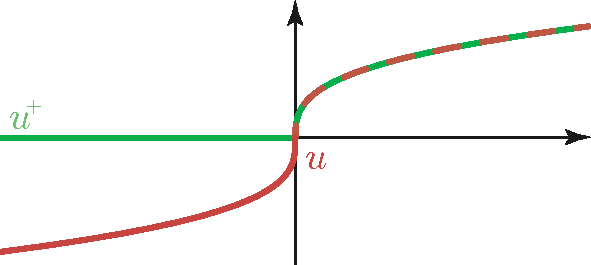
\includegraphics[trim=0cm 0cm 0cm 0cm, clip, scale=0.65]{images/partepositiva}
	\end{center}
\end{minipage}
\begin{minipage}{0.5\textwidth}
	\begin{center}
		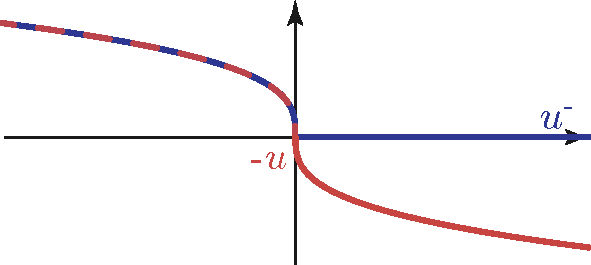
\includegraphics[trim=0cm 0cm 0cm 0cm, clip, scale=0.65]{images/partenegativa}
	\end{center}
\end{minipage}\vspace{4mm}\\
Tornando quindi a $\funz{f}{X}{\complexset}$, possiamo ottenere $f$ come combinazione lineare di quattro funzioni reali \textit{non negative}.
\begin{equation}
	f=\left(\Re f\right)+i\left(\Im f\right)=\left(\left(\Re f\right)^{+}-\left(\Re f\right)^{-}\right)+i\left(\left(\Im\right)^{+}-\left(\Im\right)^{-}\right)
\end{equation}
Con la prossima proposizione dimostreremo che le funzioni qui definite sono tutte integrabili.
\begin{proposition}[Integrabilità delle parti positive e negative delle parti reali e immaginarie]\label{integrabilitàpartiposnegrealimm}
	Se $f\in\mathcal{L}^{1}\left(\mu\right)$, allora $\left(\Re f\right)^{\pm},\ \left(\Im f\right)^{\pm}\in\mathcal{L}^{1}\left(\mu\right)$.
\end{proposition}
\begin{demonstration}
	Poiché $f\in\mathcal{L}^{1}\left(\mu\right)$, allora $\Re f$ e $\Im f$ sono misurabili; ne consegue che $\left(\Re f\right)^{\pm},\ \left(\Im f\right)^{\pm}\in\mathcal{L}^{1}\left(\mu\right)$ sono misurabili\footnote{Si vedano le ‘‘Note aggiuntive'', a pag. \pageref{misuraparterealeimm}.}, reali e non negative, dunque coincidono con il loro modulo.\\
	Poiché ogni funzione misurabile, reale, non negativa è integrabile, ciò implica che la seconda ipotesi per l'integrabilità è soddisfatta e quindi vale la tesi.
\end{demonstration}
\section{Passo 3: funzioni complesse integrabili}
Avendo enunciato tutte le premesse del caso, siamo nelle condizioni di enunciare il terzo passo dell'integrale di Lebesgue.
\begin{define}[Integrale di Lebesgue per funz. a valori complessi, integrabili]
	Sia $\funz{f}{\left(X,\mathcal{M},\mu\right)}{\complexset}$ funzione \textit{integrabile}. Posto
	\begin{equation*}
		f=\left(\Re f\right)^{+}-\left(\Re f\right)^-+i\left[\left(\Im f\right)^{+}-\left(\Im f\right)^{-}\right]
	\end{equation*}
si definisce l'\textit{integrale esteso ad E di $f$ rispetto alla misura $\mu$} come
\begin{equation}
	\int_Efd\mu\coloneqq\int_E\left(\Re f\right)^{+}d\mu-\int_E\left(\Re f\right)^{-}+i\left(\int_E\left(\Im f\right)^{+}d\mu-\int_E\left(\Im f\right)^{-}d\mu\right)
\end{equation}
\end{define}
\begin{observe}
	L'ipotesi $f\in\mathcal{L}^{1}\left(\mu\right)$ implica, come dice la proposizione \ref{integrabilitàpartiposnegrealimm}, che $\left(\Re f\right)^{\pm}$, $\left(\Im_f\right)^{\pm}\in\mathcal{L}^1\left(\mu\right)$ e quindi vale
	\begin{equation*}
		\int_X\left(\Re f\right)^{\pm}d\mu<+\infty\quad \int_X\left(\Im f\right)^{\pm}d\mu<+\infty
	\end{equation*}
	Di conseguenza, tale integrale esiste finito in $\complexset$. Se infatti le quattro funzioni ottenute decomponendo $f$ non fossero integrabili, allora potrebbero capitare delle situazioni in cui \textit{due degli integrali} della scomposizione danno la \textit{forma indeterminata} $\infty-\infty$.
\end{observe}
\begin{property}[Proprietà dell'integrale di Lebesgue per funzioni a valori in {$\complexset$}]
	Sia $\left(X,\mathcal{M},\mu\right)$ uno spazio di misura.
	\begin{enumerate}
		\item \textbf{Linearità:}
		\begin{equation}
			\int_X\left(\alpha f+\beta g\right)d\mu=\alpha\int_Xfd\mu+\beta\int_Xgd\mu,\ \forall f,g\in\mathcal{L}^1\left(\mu\right),\ \forall\alpha,\ \beta\in\complexset
		\end{equation}
		\item \textbf{Monotonia rispetto al modulo:}
		\begin{equation}
			\abs{\int_Xfd\mu}\leq \int_X\abs{f}d\mu,\ \forall f\in\mathcal{L}^1\left(\mu\right)
		\end{equation}
	\item $\sigma$-\textbf{additività rispetto al dominio:} se $\displaystyle E=\bigcup_{n\geq 1}E_n,\ \forall E_n\in\mathcal{M}\colon E_i\cap E_j=\emptyset,\ \forall i\neq j$, allora
	\begin{equation}
		f\in\mathcal{L}^1\left(\mu\right)\implies \int_Efd\mu=\sum_{n\geq 1}\int_{E_n}fd\mu
	\end{equation}
\item \textbf{Assoluta continuità:}
\begin{equation}
	f\in\mathcal{L}^{1}\left(\mu\right)\implies \forall \epsilon>0,\ \exists \delta >0\colon\forall E\in\mathcal{M}\colon \mu\left(E\right)<\delta\implies\abs{\int_E fd\mu}<\epsilon
\end{equation}
in altre parole, l'integrale si può rendere arbitrariamente più piccolo in modulo a patto di integrare su un dominio di misura sufficientemente piccola.
\end{enumerate}
\end{property}
\begin{demonstration}
	Dimostriamo l'assoluta continuità (punto 4).\\
	Consideriamo $\funz{f}{X}{\complexset}$ con $f\in\mathcal{L}^1\left(\mu\right)$; sappiamo che $f$ è misurabile e pertanto anche $\funz{\lvert f\rvert}{X}{\left[0,+\infty\right)}$ la è.\\
	Consideriamo la misura
	\begin{equation*}
		\funztot{\mu_{|f|}}{\mathcal{M}}{\left[0,+\infty\right]}{E}{\int_E\abs{f}d\mu}
	\end{equation*}
Essa è assolutamente continua rispetto a $\mu$. Inoltre, $\mu_{\abs{f}}$ è finita perché $f\in\mathcal{L}^1\left(\mu\right)$ e quindi
\begin{equation*}
	\mu_{\abs{f}}(x)\int_X\abs{f}d\mu<+\infty
\end{equation*}
Per la caratterizzazione delle misure finite assolutamente continue rispetto a $\mu$ si ha
\begin{equation*}
	\forall \epsilon >0,\ \exists \delta > 0\colon E\in\mathcal{M},\ \mu\left(E\right)<\delta\implies \mu_{\abs{f}}\left(E\right)=\int_E\abs{f}d\mu<\epsilon
\end{equation*}
Si ha quindi
\begin{equation*}
	\forall \epsilon > 0,\ \exists \delta >0\colon \exists E\in\mathcal{M},\ \mu\left(E\right)<\delta\implies \abs{\int_Efd\mu}\underset{\substack{\text{prop. }2\\\text{dell'int.}}}{\leq}\int_E\abs{f}d\mu<\epsilon\implies \abs{\int_Efd\mu}<\epsilon\qedhere
\end{equation*}
\end{demonstration}
\subsection{Teorema della convergenza dominata}\index{teorema!della convergenza dominata}
\begin{theorema}[Teorema della convergenza dominata]\label{thmconvergenzadominata}
Sia $\left(X,\mathcal{M},\mu\right)$ uno spazio di misura e $\funz{f_n}{X}{\complexset}$ una successione di funzioni misurabili tale che esiste
\begin{equation*}
	f(x)=\lim_{n\to+\infty}f_n(x),\ \forall x\in X
\end{equation*}
Se esiste una funzione $g\in \mathcal{L}^{1}\left(\mu\right)$ tale per cui
\begin{equation*}
	\abs{f_n(x)}\leq g(x),\ \forall n\geq 1,\ \forall x\in X
\end{equation*}
allora $f\in \mathcal{L}^{1}\left(\mu\right)$ e vale
\begin{equation}
	\lim_{n\to+\infty}\int_X\abs{f_n-f}d\mu=0
\end{equation}
e vale il \textbf{passaggio al limite sotto segno di integrale}\index{passaggio al limite sotto segno di integrale}:
\begin{equation}
	\lim_{n\to+\infty}\int_Xf_nd\mu=\int_Xfd\mu
\end{equation}
\end{theorema}
\begin{demonstration}
	Poiché $f_n$ è una successione di funzioni misurabili che converge puntualmente a $f$, $\forall x\in X$, $f$ è una funzione misurabile. Inoltre, dato che tutti gli elementi della successione $f_n$ sono maggiorati (in modulo) da $g$, si ha per monotonia del limite che
	\begin{equation*}
		\circled[red]{\vardiamond}\quad \abs{f}\leq g
	\end{equation*}
	Allora, applicando i moduli ai membri della disequazione vale $\abs{f}\leq\abs{g}$. Integrando rispetto a Lebesgue, per monotonia rispetto all'integranda si ha
	\begin{equation*}
		\int_X\abs{f}d\mu\leq \int_X \abs{g}d\mu<+\infty
	\end{equation*}
	in quanto $g\in \mathcal{L}^1\left(\mu\right)$; segue che $f\in \mathcal{L}^1\left(\mu\right)$.\\
	Osserviamo che
	\begin{align*}
		\abs{f_n-f}&\leq \abs{f_n}+\abs{f}&\text{(disuguaglianza triangolare)}\\
		&\leq2g&\text{(per $\circled[red]{\vardiamond}$)}
	\end{align*}
	da cui segue che $2g-\abs{f_n-f}\geq 0$ e quindi sono funzioni non negative. Poiché le $2g-\abs{f_n-f}$ sono misurabili in quanto somma di funzioni in $\mathcal{L}^1\left(\mu\right)$ (e quindi misurabili), possiamo applicare il \textit{lemma di Fatou} a tali funzioni e ottenere
	\begin{gather*}
		\int_X\left(\liminf_{n\to+\infty}2g-\abs{f_n-f}\right)d\mu\leq\liminf_{n\to+\infty}\int_X\left(2g-\abs{f_n-f}\right)d\mu\\
		\viff\\
		\int_X 2gd\mu-\int_X\liminf_{n\to+\infty}\abs{f_n-f}d\mu\leq\int_X 2gd\mu+\liminf_{n\to+\infty}\left(-\int_X\abs{f_n-f}d\mu\right)
	\end{gather*}
	ma
	\begin{equation*}
		\int_X\liminf_{n\to+\infty}\abs{f_n-f}d\mu=0
	\end{equation*}
	in quanto per ipotesi $\displaystyle\lim_{n\to+\infty}f_n=f\iff\lim_{n\to+\infty}\abs{f_n-f}=0$; segue che $\liminf$ e $\lim$ coincidono con valore $0$ e pertanto anche l'integrale risulta nullo.\\
	Inoltre, notiamo che
	\begin{equation*}
		\int_X\abs{f_n-f}d\mu
	\end{equation*}
	è una successione a valori non negativi, dunque per le proprietà del massimo e minimo limite\footnote{Nelle ‘‘Note aggiuntive'', a pag. \pageref{maxminlegame} è possibile trovare la dimostrazione di questo risultato insieme ad altri relativi al limsup e liminf.} si ha
	\begin{equation*}
		\liminf_{n\to+\infty}\left(-\int_X\abs{f_n-f}d\mu\right)=-\limsup_{n\to+\infty}\left(\int_X\abs{f_n-f}d\mu\right)
	\end{equation*}
	Allora otteniamo
	\begin{equation*}
		\int_X 2gd\mu\leq\int_X 2gd\mu-\limsup_{n\to+\infty}\left(\int_X\abs{f_n-f}d\mu\right)
	\end{equation*}
	Dato che $g\in \mathcal{L}^1\left(\mu\right)$ è non negativa, si ha  
	\begin{equation*}
		\int_X2gd\mu=2\int_X\abs{g}d\mu<+\infty
	\end{equation*}
	Possiamo dunque sottrarre
	\begin{equation*}
		\int_X 2gd\mu
	\end{equation*}
	da entrambi i membri della disequazione e ottenere
	\begin{equation*}
		\circled[blue]{\spadesuit}\quad \limsup_{n\to+\infty}\int_X\abs{f_n-f}d\mu\leq 0
	\end{equation*} 
	Notiamo che se una successione di numeri reali non negativi non converge a $0$, allora il massimo limite è positivo.\footnote{Infatti, se $a_n\geq 0,\ \forall n\in\naturalset$, allora anche il limite $\displaystyle \lim_{n\to+\infty}a_n$ sarà non negativo.  Tuttavia, poiché tale successione ammette limite, allora esso coincide con il suo massimo limite. Segue immediatamente che
	\begin{equation*}
		\lim_{n\to+\infty}a_n\neq0\implies \lim_{n\to+\infty}a_n>0\implies \limsup_{n\to+\infty}a_n>0
	\end{equation*}} Per contronominale, se il massimo limite di numeri reali non negativi \textit{non} è positivo, allora la serie converge a $0$ necessariamente. Poiché vale \circled[blue]{\spadesuit}, allora ciò implica la prima tesi:
	\begin{equation*}
		\lim_{n\to+\infty}\int_X\abs{f_n-f}d\mu=0
	\end{equation*}
	Infine, poiché l'integrale di Lebesgue è monotono rispetto al modulo, si ha
	\begin{equation*}
		0=\lim_{n\to+\infty}\int_X\abs{f_n-f}d\mu\geq\lim_{n\to+\infty}\abs{\int_X\left(f_n-f\right)d\mu}\ge 0
	\end{equation*}
	e quindi
	\begin{equation*}
		\lim_{n\to+\infty}\abs{\int_X \left(f_n-f\right)d\mu}=0\implies\lim_{n\to+\infty}\int_X\left(f_n-f\right)d\mu=0\implies\lim_{n\to+\infty}\int_X f_nd\mu=\int_X fd\mu
	\end{equation*}
	ottenendo la seconda e ultima tesi.
\end{demonstration}
\section{Tra integrale di Riemann e integrale di Lebesgue}
Nell'excursus storico abbiamo visto come l'\textit{integrale di Lebesgue} e le sue successive astrazioni di inizio '900 siano state la risposta a due domande che indirizzarono gli studi di Analisi del XIX secolo:
\begin{itemize}
	\item Come si può allargare la classe delle funzioni integrabili?
	\item Come si può caratterizzare l'insieme dei punti di discontinuità di una funzione integrabile secondo Riemann?
\end{itemize}
Con i tre passi precedentemente esposti abbiamo costruito l'integrale astratto di Lebesgue e risposto alla prima domanda, mentre rimane al momento aperta la seconda; in particolare, nel caso di funzioni da $\realset$ a $\realset$, sorge la questione: \textit{che relazione c'è tra l'integrale di Riemann e l'integrale di Lebesgue?}\\
Nel caso di funzioni limitate su un intervallo chiuso e che sono Riemann-integrabili scopriamo che tali integrali coincidono.
\begin{theoremaqed}[Integrale proprio di Riemann implica integrale di Lebesgue]
	Sia $\funz{f}{\left[a,b\right]}{\realset}$ limitata e misurabile. Allora
	\begin{equation}
		f\in\mathcal{R}\left(\left[a,b\right]\right)\implies f\in\mathcal{L}^1\left(\left[a,b\right],m_1\right)
	\end{equation}
e
\begin{equation}
	\int_{\left[a,b\right]}\abs{f}dm_1=\int_{a}^{b}f(x)dx\qedhere
\end{equation}
\end{theoremaqed}
% TO DO: add cenni dimostrazione
\begin{observes}~
	\begin{itemize}
		\item Il viceversa non è vero: come abbiamo già visto\footnote{Si veda pag. \pageref{funzionedirichletintegrale}.}, la funzione di Dirichlet è integrabile secondo Lebesgue ma non secondo Riemann.
		\item L'ipotesi di misurabilità è in realtà ridondante: come si potrà vedere con i risultati della sezione successiva, ogni funzione limitata e Riemann-integrabile è sempre misurabile rispetto alla misura di Lebesgue $m_1$.
	\end{itemize}
\end{observes}
Situazione differente si ha con l'integrale improprio di Riemann: infatti, può capitare che ci siano funzioni integrabili (almeno impropriamente) secondo Riemann ma \textit{non} secondo Lebesgue!
\begin{theoremaqed}[Integrale improprio di Riemann e integrale di Lebesgue]\label{integraleimproprioriemannlebesgue}
	Sia $\funz{f}{\left[a,+\infty\right]}{\realset}$ misurabile tale che $f\in\mathcal{R}\left(\left[a,b\right]\right)$ per ogni $b>a$. Allora
	\begin{enumerate}
		\item Vale la relazione
		\begin{equation}
			\int_{\left[a,+\infty\right)}\abs{f}dm_1=\int_{0}^{+\infty}\abs{f(x)}dx\in\left[0,+\infty\right]
		\end{equation}
		\item Se l'integrale improprio di Riemann di $f$ su $\left[a,+\infty\right)$ converge \textit{assolutamente} allora $f$ è integrabile secondo Lebesgue su $\left[a,+\infty\right)$ e
		\begin{equation}
			\int_{\left[a,+\infty\right)}fdm_1=\int_{a}^{+\infty}f(x)dx\in\realset\qedhere
		\end{equation}
	\end{enumerate}
\end{theoremaqed}
\begin{observe}
	Se l'integrale improprio di Riemann di $f$ su $\left[a,+\infty\right)$ converge ma non \textit{assolutamente} allora $f$ \textit{non} è integrabile secondo Lebesgue su $\left[a,+\infty\right)$.
\end{observe}
\begin{example}
	Consideriamo la funzione
	\begin{equation*}
		f(x)=\frac{\sin x}{x}
	\end{equation*}
	sull'intervallo $\left[\pi,+\infty\right)$. Mostriamo che:
	\begin{enumerate}
		\item L'integrale di $f$ secondo Riemann converge semplicemente.
		\item L'integrale di $f$ secondo Riemann \textit{non} converge assolutamente.
		\item La funzione $f$ \textit{non} è integrabile secondo Lebesgue.
	\end{enumerate}
\begin{enumerate}[label=\Roman*]
	\item Integrando per parti si ha
	\begin{align*}
		\int_{\pi}^{+\infty}\frac{\sin x}{x}dx&=\lim_{R\to+\infty}\int_{\pi}^{R}\frac{\sin x}{x}dx=\lim_{R\to+\infty}\left[-\frac{\cos x}{x}\Big|^{R}_{\pi}-\int_{\pi}^{R}\frac{\cos x}{x^2}dx\right]\\
		&=\lim_{R\to+\infty}\biggl[\underbrace{-\frac{\cos R}{R}}_{\substack{\to 0\text{ per}\\R\to+\infty}}+\cos \pi-\int_{\pi}^{R}\frac{\cos x}{x^2}dx\biggr]=-1-\int_{\pi}^{+\infty}\frac{\cos x}{x^2}dx
	\end{align*}
dato che
\begin{equation*}
	0\leq \abs{\frac{\cos x}{x^2}}\leq \frac{1}{x^2}
\end{equation*}
e
\begin{equation*}
	\int_{\pi}^{\infty}\frac{1}{x^2}
\end{equation*}
converge, allora
\begin{equation*}
	\int_{\pi}^{+\infty}\abs{\frac{\cos x}{x^2}}
\end{equation*}
converge e dunque
\begin{equation*}
	\int_{\pi}^{+\infty}\frac{\sin x}{x}dx
\end{equation*}
converge (assolutamente). Ne consegue che l'integrale di $f(x)$ è \textit{semplicemente convergente}.
\item Osserviamo che, per ogni $n\in\naturalset$, si ha
\begin{align*}
	\int_{\pi}^{n\pi}\frac{\abs{\sin x}}{x}dx&=\sum_{k=1}^{n-1}\int_{k\pi}^{\left(k+1\right)\pi}\frac{\abs{\sin x}}{x}dx&\\
	&>\sum_{k=1}^{n-1}\frac{1}{\left(k+1\right)\pi}\int_{k\pi}^{\left(k+1\right)\pi}\abs{\sin x}dx&\text{($\nicefrac{1}{x}$ decrescente)}\\
	&=\sum_{k=1}^{n-1}\frac{2}{\left(k+1\right)\pi}=\frac{2}{\pi}\sum_{k=2}^{n}\frac{1}{k}&
\end{align*}
operando nell'ultimo passaggio un cambio di indice $k-1\to k$. Passando al limite per $n\to+\infty$ si ha
\begin{equation*}
	\int_{\pi}^{+\infty}\frac{\abs{\sin x}}{x}dx>\frac{2}{\pi}\sum_{k=2}^{+\infty}\frac{1}{k}=\frac{2}{\pi}\left[\sum_{k=1}^{+\infty}\frac{1}{k}-1\right]
\end{equation*}
Poiché l'integrale è minorato dalla \textit{serie armonica}, che sappiamo essere \textit{divergente}, allora l'integrale diverge e quindi l'integrale della funzione $f(x)$ \textit{non} converge \textit{assolutamente}.
\item Per il primo punto del teorema \ref{integraleimproprioriemannlebesgue} vale
\begin{equation*}
	\int_{\left[\pi,+\infty\right)}\abs{\frac{\sin x}{x}}dm_1=\int_{\pi}^{\infty}\abs{\frac{\sin x}{x}}dx=+\infty
\end{equation*}
Poiché l'integrale improprio di Riemann \textit{non} converge assolutamente, segue che $f$ non è integrabile su $\left[\pi,+\infty\right)$ e pertanto non ammette integrale secondo Lebesgue.
\end{enumerate}
\end{example}
Sulla base di questi risultati siamo finalmente in grado di rispondere al secondo quesito: con una certa ironia, la caratterizzazione dell'insieme dei punti di discontinuità di una funzione integrabile secondo Riemann è basata sulla \textbf{misura di Lebesgue}.
\begin{theoremaqed}[Caratterizzazione delle funzioni integrabili secondo Riemann]
	Sia $\funz{f}{\left[a,b\right]}{\realset}$ limitata e sia $D_f$ l'insieme delle discontinuità di $f$. Se $m_1$ è la misura  di Lebesgue unidimensionale, allora
	\begin{equation}
		f\in\mathcal{R}\left(\left[a,b\right]\right)\iff m_1\left(D_f\right)=0\qedhere
	\end{equation}
ossia $f$ limitata è Riemann-integrabile su $\left[a,b\right]$ se e solo se $f$ è continua \textbf{q.o.} su $\left[a,b\right]$.
\end{theoremaqed}
\begin{example}
	Sia $C\subseteq\left[0,1\right]$ l'insieme di Cantor e sia $f=\chi_C$ la funzione caratteristica su tale insieme.
	Si ha che $D_f=\partial C$, ma poiché $C$ è un chiuso con interno vuoto, allora
	\begin{equation*}
		D_f=\partial C=C
	\end{equation*}
	Essendo $m_1\left(C\right)=0$, $f$ è integrabile secondo Riemann su $\left[0,1\right]$.
\end{example}
\section{Il ruolo degli insiemi di misura nulla}
Abbiamo appena visto come una funzione è integrabile secondo Riemann se e solo se l'insieme delle sue discontinuità è un insieme di misura nulla. In altre parole, una funzione è integrabile secondo Riemann su un dato intervallo se e solo se essa è continua, tolto al più un insieme misurabilmente nullo di discontinuità.\\
Più in generale, ha senso parlare di proprietà valide su un particolare dominio tolto un insieme di misura nulla: poiché queste proprietà non valgono su insiemi la cui \textit{rilevanza è minima}, quantomeno dal punto della \textit{misura}, possiamo definire tale proprietà come \textit{quasi ovunque valida}.
\begin{define}[Proprietà quasi ovunque valida]
	Sia $\left(X,\mathcal{M},\mu\right)$ uno spazio di misura. Si dice che una proprietà $P$ vale \textbf{‘‘quasi ovunque''} (\textbf{q.o.})\index{proprietà quasi ovunque valida} o ‘‘$\mu$\textbf{-quasi ovunque}'' se vale in tutto $X$ tranne eventualmente su un insieme di misrua $\mu$ nulla. In altre parole, deve esistere un insieme $N\in\mathcal{M}$ con $\mu(N)=0$ tale che $\forall x\in X\setminus N$ vale tale proprietà $P$.
\end{define}
\begin{observe}
	Dalla definizione in sè \textit{non} è richiesto che l'insieme $E=\{x\in\ X\mid P(x)\text{non vale}\}$ sia misurabile, ma solamente che sia contenuto in un insieme misurabile e di misura nulla.\\
	Tuttavia, se la misura è \textit{completa}, allora anche $E$ risulta essere misurabile e di misura nulla.
\end{observe}
\begin{examplewt}[Uguaglianza quasi ovunque]
	Siano $\funz{f,g}{X}{\complexset}$ misurabili. Allora
	\begin{equation}
		f=g\ \text{\textbf{q.o.}}\iff \text{Posto}\ E=\{x\in\ X\mid f(x)\neq g(x)\},\ \mu\left(E\right)ù=0
	\end{equation}
	Poiché $E=(f-g)^{-1}\left(\complexset\setminus\{0\}\right)$, $f,\ g$ sono misurabili e $\complexset\setminus\{0\}$ è aperto, allora $E$ è misurabile e la definizione è ben posta.\\
	Inoltre, si può notare che si può estendere la stessa definizione di uguaglianza \textbf{q.o.} a funzioni $f,\ g$ \textit{non} necessariamente misurabili con codominio uno spazio topologico, a patto di supporre che la misura $\mu$ sia \textit{completa}.
\end{examplewt}
\begin{example}
	Consideriamo la funzione di Dirichlet $f=\chi_{\left[0,1\right]\cap\rationalset}$:
	\begin{equation*}
		f(x)=\begin{cases}
			\begin{array}{ll}
				1&\text{se }x\in\left[0,1\right]\cap\rationalset\\
				0&\text{se }x\in\left[0,1\right]\setminus\rationalset
			\end{array}
		\end{cases}
	\end{equation*}
Sappiamo che $m_1\left(\left[0,1\right]\cap\rationalset\right)=0$, quindi
\begin{equation*}
	\left\{x\in\left[0,1\right]\mid f(x)\neq 0\right\}=\left[0,1\right]\cap \rationalset
\end{equation*}
ha misura nulla e pertanto la funzione di Dirichlet è \textit{quasi ovunque} la funzione identicamente \textit{nulla}.
\end{example}
\begin{property}[Ruolo degli insiemi di misura nulla nell'integrazione]
Sia $\left(X,\mathcal{M},\mu\right)$ uno spazio di misura. Allora
\begin{enumerate}
	\item Se $\funz{f}{X}{\complexset}$ e $f\in\mathcal{L}^{1}\left(\mu\right)$, allora
	\begin{equation}
		\forall E\in\mathcal{M},\ \mu\left(E\right)=0\implies \int_Efd\mu=0
	\end{equation}
\item Se $\funz{f,g}{X}{\complexset}$ e $f,g\in\mathcal{L}^{1}\left(\mu\right)$, allora
\begin{equation}
	f=g\ \text{\textbf{q.o.}}\implies \int_Xfd\mu=\int_Xgd\mu
\end{equation}
\item Se $\funz{f}{X}{\left[0,+\infty\right)}$ misurabile, allora
\begin{equation}
	\int_X fd\mu=0\implies f=0 \text{\textbf{q.o.} in }X
\end{equation}
\end{enumerate}
\end{property}
\begin{demonstration}~{}
	\begin{enumerate}[label=\Roman*]
		\setcounter{enumi}{1}
		\item Posto
		\begin{equation*}
			E=\left\{x\in X\mid f(x)\neq g(x)\right\}
		\end{equation*}
	si ha $\mu\left(E\right)=0$. Allora
	\begin{equation*}
		\int_Xfd\mu=\int_{X\setminus E}fd\mu+\int_Efd\mu=\int_{X\setminus E}gd\mu+0=\int_{X\setminus E}gd\mu+\int_Egd\mu=\int_Xgd\mu
	\end{equation*}
	\item Sia
		\begin{equation*}
			E=\left\{x\in X\mid f(x)\neq 0\right\}=\bigcup_{n\geq 1}\left\{x\in X\mid f(x)>\frac{1}{n}\right\}=\bigcup_{n\geq 1}E_n
		\end{equation*}
	Osserviamo che $E_n=f^{-1}\left(\left(\frac{1}{n},+\infty\right)\right)\in\mathcal{M}$ in quanto è controimmagine di un aperto tramite una funzione misurabile; su ha allora
	\begin{align*}
		0&=\int_Xfd\mu&\\
		 &\leq\int_{E_n}fd\mu&\text{(monotonia dell'integrale rispetto al dominio)}\\
		 &\leq\int_{E_n}\frac{1}{n}d\mu&\text{(monotonia rispetto l'integranda)}\\
		 &=\frac{1}{n}\mu\left(E_n\right)\leq 0&
	\end{align*}
	Segue dunque che $\mu\left(E_n\right)=0,\ \forall n\geq 1$; utilizzando la $\sigma$-subadditività della misura vediamo che
	\begin{equation*}
		\mu\left(E\right)=\mu\left(\bigcup_{n\geq 1}E_n\right)\leq\sum_{n=1}^{+\infty}\mu\left(E_n\right)=0\implies \mu\left(E\right)=0
	\end{equation*}
	Vale dunque la tesi.\qedhere
	\end{enumerate}
\end{demonstration}
Avendo definito il concetto di proprietà quasi ovunque valida, possiamo enunciare un'altra versione dello \textit{scambio tra integrale e serie}, questo risultato che segue dal \textit{teorema della convergenza dominata}.
\begin{theorema}[Scambio tra integrale e serie per funzioni integrabili]
	Sia $\left(X,\mathcal{M},\mu\right)$ uno spazio di misura. Siano $\funz{f_n}{X}{\complexset}$ integrabili. Supponiamo che
	\begin{equation*}
		\sum_{n=1}^{+\infty}\int_X\abs{f_n}d\mu<+\infty
	\end{equation*}
Allora
\begin{enumerate}
	\item $\displaystyle f(x)=\sum_{n=1}^{+\infty}f_n(x)$ è definita \textbf{q.o.} in $X$.
	\item $f\in\mathcal{L}^{1}\left(\mu\right)$
	\item Vale lo \textit{scambio tra integrale e serie}\index{scambio tra integrale e serie}:
	\begin{equation}
		\int_Xfd\mu=\int_X\left(\sum_{n=1}^{+\infty}f_n\right)d\mu=\sum_{n=1}^{+\infty}\int_Xfd\mu\in\complexset
	\end{equation}
\end{enumerate}
\end{theorema}